\documentclass{article}
% T1 encoding lets the Times/Courier of the `times' package load under
% both pdfTeX and XeTeX-based builds (tectonic); without it XeTeX silently
% falls back to Latin Modern and drops every bold and monospace shape.
\usepackage[T1]{fontenc}
\usepackage{iclr2027_conference,times}
% \iclrfinalcopy   % uncomment for the camera-ready

\usepackage{amsmath,amssymb,amsthm}
\usepackage{booktabs}
\usepackage{multirow}
\usepackage{tabularx}
\usepackage{graphicx}
\usepackage{flafter}
\usepackage{placeins}
\usepackage{listings}
\usepackage{algorithm}
\usepackage{algpseudocode}
\usepackage{tikz}
\usetikzlibrary{positioning,arrows.meta,fit,calc}
\usepackage{xcolor}
\usepackage[most]{tcolorbox}
\usepackage[hidelinks]{hyperref}
\usepackage{url}

\lstset{basicstyle=\ttfamily\footnotesize, breaklines=true,
  columns=fullflexible, keepspaces=true}
\newtcolorbox{promptbox}[1]{colback=gray!6, colframe=black!60,
  title={#1}, fonttitle=\bfseries\small, breakable, boxrule=0.6pt,
  left=4pt, right=4pt, top=4pt, bottom=4pt}

% ---- figure palette (colour-blind safe, print-legible) ----
\definecolor{achieve}{RGB}{31,119,120}
\definecolor{refute}{RGB}{178,58,50}
\definecolor{bdh}{RGB}{110,110,118}

% Five floats in one section otherwise pile up and drift pages away from
% the text that discusses them; loosen the default placement limits.
\renewcommand{\topfraction}{0.85}
\renewcommand{\bottomfraction}{0.5}
\renewcommand{\textfraction}{0.08}
\renewcommand{\floatpagefraction}{0.75}
\setcounter{topnumber}{2}
\setcounter{bottomnumber}{1}
\setcounter{totalnumber}{3}

\newcommand{\algdelta}[1]{\begingroup\setlength{\fboxsep}{0.65pt}\colorbox{achieve!13}{#1}\endgroup}
\newcommand{\algside}[1]{\Comment{\parbox[t]{.34\linewidth}{\raggedright\footnotesize #1}}}

\newtheorem{theorem}{Theorem}
\newtheorem{lemma}[theorem]{Lemma}
\newcommand{\F}{\mathbb{F}}
\newcommand{\vct}[1]{\boldsymbol{#1}} % vectors; coordinates and coefficients remain scalar
\newcommand{\wt}{\operatorname{wt_s}}
\newcommand{\cmins}{c^{\mathrm{s}}_{\min}}
\newcommand{\claim}[1]{\textbf{\texttt{#1}}}   % auditor claim names

\title{Reproducible LLM-Guided Discovery of\\
  Entanglement-Assisted Quantum Codes}
\author{Anonymous authors \\ Paper under double-blind review}

\begin{document}
\maketitle

\begin{abstract}
LLM-guided program evolution can produce mathematical constructions, but
verifying a result and reproducing the search that produced it are
separate requirements. We study both for entanglement-assisted quantum
error-correcting codes (EAQECCs), using targets derived from tabulated
EAQECC bounds and an exact symplectic evaluator. The core construction archive
contains 115 verified codes, a closed-form construction
$[[n,1,n-1;n-q-1]]_q$ for every prime power at the stated admissible
lengths, and ten nonexistence results backed by DRAT certificates.
The construction and ebit lifting settle 54 listed gaps; applying the
known EA-Plotkin bound tightens 398 listed upper bounds. An auditor
checks the archived computational results and replays fixed search
programs using an evaluation-based stopping rule. It does not reproduce
the LLM sampling that generated those programs. The pipeline supports researcher proposals that change the search
representation and can be developed through program-level feedback.
Under identical guidance to search the symplectic dual, a four-block
comparison increases held-out success from 50.0\% to 68.8\% at $n=9$
and from 15.6\% to 50.0\% at $n=11$ when independent proposals are
replaced by iterative program development. One validation-selected
later-generation program achieves 75.0\% success at each of $n=13,15$.
\end{abstract}

%==============================================================
\section{Introduction}
%==============================================================

LLM-guided program search has produced new mathematical constructions
and algorithms~\citep{FunSearch,AlphaEvolve}. Assessing such results
requires answering three questions: whether the proposed object is
valid, whether it improves on prior constructions, and what the model
contributed beyond the initial program and task specification. These
questions require different evidence. A verified output does not by
itself establish novelty, and rerunning a final program does not
reproduce the evolutionary process that generated it.

We study these distinctions using entanglement-assisted quantum
error-correcting codes (EAQECCs). Their parameters can be computed
exactly from a finite list of generators, while tabulated EAQECC bounds
provide a specific reference for measuring improvements. Figure~\ref{fig:overview} summarizes our researcher-guided pipeline
for program evolution, exact verification and nonexistence checking.
The artifact records the mathematical results and the evidence needed
to check each type of claim.

Several improvements concern constructions published in 2020 and 2022
that remained listed in the EAQECC tables accessed on 17 July
2026~\citep{GHW2020,Luo2022}. Our constructions and certified exclusions
close nine previously tabulated qubit distance gaps (Table~\ref{tab:results}).
The prior constructions predate our table access by approximately four
to six years. Their dates document available constructions rather than
a complete history of improvement attempts.

\paragraph{Contributions.}
\begin{itemize}\setlength{\itemsep}{1pt}
\item \textbf{A search problem with explicit verification criteria.}
  We construct targets from tabulated EAQECC bounds. The archived qubit
  table contains 563 entries whose distance bounds differ by one.
  We distinguish closing a listed gap, improving a lower bound and
  constructing a code at a parameter cell absent from the table
  (Section~\ref{sec:related}).
\item \textbf{A researcher-guided pipeline and reproduction protocol.}
  Researchers can revise construction ideas and campaign targets through
  archived task specifications. The auditor checks codes, family
  instances, table comparisons, nonexistence evidence and prompt provenance. A virtual
  clock tied to evaluator calls makes fixed-program search replayable
  under an evaluation-based stopping rule; negative controls test
  the auditor's response to damaged inputs (Section~\ref{sec:repro}).
\item \textbf{EAQECC constructions and nonexistence results.}
  A closed form at distance $n-1$ settles 54 listed gaps, including
  qutrit entries obtained by ebit lifting. We also archive finite
  codes using less entanglement and nonexistence results that
  establish minimum entanglement at specified lengths. Applying the
  known EA-Plotkin bound tightens 398 listed upper bounds
  (Tables~\ref{tab:results} and~\ref{tab:results-qudit}).
\item \textbf{Research-guided program development with measured outcomes.}
  Two generation policies receive the same initial program and researcher
  proposal to search the symplectic dual. Iterative development achieves
  higher mean held-out success than independent proposals, with the
  larger difference at length 11. A selected later-generation program
  also generalizes to lengths 13 and 15 (Section~\ref{sec:ablation}).
\end{itemize}

%==============================================================
\section{Background and related work}\label{sec:related}
%==============================================================

\subsection{Entanglement-assisted quantum error-correcting codes}
\label{sec:ea-background}

Quantum error correction protects quantum information sent through noisy
communication links. Early stabilizer constructions imposed algebraic
compatibility constraints that limited which classical codes could be
reused. \citet{BrunDevetakHsieh2006} showed that entanglement shared in
advance between sender and receiver relaxes these constraints, enabling
a broader class of quantum codes. This is the motivation for
entanglement-assisted quantum error-correcting codes (EAQECCs).

A code with parameters $[[n,k,d;c]]_q$ encodes $k$ logical qudits into
$n$ transmitted $q$-level systems using $c$ shared maximally entangled
qudit pairs. Each pair contains $\log_2 q$ ebits, equal to one for
qubits ($q=2$)~\citep{GHW2022}. The receiver's
halves are assumed noiseless and are not counted in $n$.

The distance $d$ determines the code's guaranteed error protection.
With ideal decoding, it corrects arbitrary errors on up to
$\lfloor(d-1)/2\rfloor$ transmitted qudits, or up to $d-1$
\emph{erasures}, where the lost qudits' locations are
known~\citep{BrunDevetakHsieh2006,GHW2022}. Increasing $d$ at fixed
$(q,n,k,c)$ strengthens protection without increasing the transmission or
entanglement budget. For example, our $[[12,1,11;8]]_2$ code raises
the listed distance from 9 to 11, increasing the guaranteed correction
of arbitrary errors from four to five transmitted qubits with the same
resources (Table~\ref{tab:results}). A verified code thus provides an
encoding specification for a quantum link with given resource and
error-protection requirements. Reducing $c$ at fixed $(n,k,d)$ instead
lowers the entanglement needed before transmission~\citep{Luo2022}.

\subsection{Code discovery as program search}
\label{sec:tables-search-background}

We search linear stabilizer EAQECCs represented by generator matrices
over $\F_q$. The LLM revises a search program that proposes matrices;
an exact evaluator computes their $(k,c,d)$. At fixed $(q,n,k,c)$,
reference tables give a constructed lower distance bound $d_\ell$ and
an upper bound $d_u$~\citep{Codetables,Luo2022}. Finding $d>d_\ell$
improves the lower bound, while reaching $d_u$ closes the gap.
We also construct codes at unlisted cells and minimize entanglement,
denoted $\cmins(n,k,d)$ within our stabilizer class. Applicable bounds
filter impossible targets~\citep{GHW2022}; Appendix~\ref{app:domain}
gives the representation, notation and comparison rules.

\textsc{FunSearch} evolves programs that construct mathematical objects or
make algorithmic decisions, using an evaluator to select useful revisions.
It produced larger cap-set constructions and improved online bin-packing
heuristics~\citep{FunSearch}; its executable outputs let researchers inspect
and develop the underlying mathematical ideas. \textsc{AlphaEvolve}
extends this approach to matrix-multiplication algorithms, data-center
scheduling, hardware-circuit simplification and model-training
kernels~\citep{AlphaEvolve,Georgiev2025}. Related frameworks include
\textsc{OpenEvolve}, \textsc{CodeEvolve}, \textsc{ShinkaEvolve} and
\textsc{TurboEvolve}, which implement or extend evaluator-guided program
evolution with population management and proposal-selection
strategies~\citep{OpenEvolve,CodeEvolve,ShinkaEvolve,TurboEvolve}.
We use \textsc{AlphaEvolve} as the evolution engine for EAQECC discovery,
supplying target parameters, an exact evaluator and researcher-directed
construction ideas.

Quantum-code discovery also uses genetic algorithms to evolve stabilizer
representations~\citep{WebsterBrowne2024}, and reinforcement learning to
optimize codes and encoders~\citep{Nautrup2019,Su2023,Mauron2023,Olle2024}.
More directly, \citet{CruzBenito2026} evolve Python generators for
bivariate bicycle codes, verify candidates, and derive structural results.
Our contribution concerns EAQECC distance--entanglement targets: exact
finite-field evaluation supports finite constructions, a prime-power
family with a Lean-checked algebraic certificate, and certified
nonexistence results. The controlled study compares independent proposals
with iterative program feedback under a shared researcher proposal.


%==============================================================
\section{The discovery pipeline}\label{sec:pipeline}
%==============================================================

Our discovery pipeline combines human-in-the-loop (HITL) research with
LLM-guided program evolution and exact verification. Researchers propose
construction ideas, inspect verified instances and revise the task between
campaigns. Figure~\ref{fig:overview} connects these interventions to the
automated search and evaluation loop. Constructed codes establish lower
distance bounds; SAT refutations with checked certificates lower upper
bounds. Independent verification and archived evidence support both routes.
The resulting constructions can inform further searches and human
mathematical generalization.

% GENERATED by scripts/make_pipeline_overview.py.
\begin{figure}[H]
\centering
\resizebox{\linewidth}{!}{% GENERATED by scripts/make_pipeline_overview.py; edit the generator.
\definecolor{ovink}{HTML}{203849}%
\definecolor{ovblue}{HTML}{2C5F8A}%
\definecolor{ovteal}{HTML}{1F7778}%
\definecolor{ovhuman}{HTML}{985B23}%
\definecolor{ovred}{HTML}{A54339}%
\begin{tikzpicture}[x=1cm,y=1cm,>=Latex,
  font=\rmfamily\fontsize{9.2}{10.8}\selectfont,text=ovink,
  flow/.style={->,draw=ovink!85,line width=.95pt},
  humanflow/.style={->,draw=ovhuman,line width=.95pt,dashed},
  small/.style={font=\rmfamily\fontsize{8.2}{9.8}\selectfont},
  label/.style={font=\rmfamily\bfseries\fontsize{9.2}{10.5}\selectfont},
  card/.style={rounded corners=3pt,draw=ovink!40,line width=.75pt,fill=white}]
\path[use as bounding box] (-.03,.24) rectangle (14.03,7.00);

% Research work is outside the automated candidate-evaluation loop.
\begin{scope}[yshift=.65cm]
\filldraw[rounded corners=4pt,fill=ovhuman!6,draw=ovhuman!40,line width=.65pt]
  (0,5.18) rectangle (14,6.32);
\fill[ovhuman!12] (.17,5.34) rectangle (2.91,6.16);
\draw[ovhuman,line width=1pt] (.53,5.91) circle (.10);
\draw[ovhuman,line width=1pt,rounded corners=2pt] (.34,5.53) -- (.34,5.66)
  .. controls (.36,5.83) and (.70,5.83) .. (.72,5.66) -- (.72,5.53);
\node[label,anchor=west,text=ovhuman] at (.88,5.94) {Researcher};
\node[small,anchor=west,text=ovhuman] at (.88,5.58) {HITL};
\node[label,anchor=west] at (3.2,5.96) {Propose ideas};
\node[small,anchor=west] at (3.2,5.57) {e.g., cyclic shifts};
\node[label,anchor=west] at (6.65,5.96) {Interpret discoveries};
\node[small,anchor=west] at (6.65,5.57) {generalize and prove};
\node[label,anchor=west] at (10.33,5.96) {Revise the task};
\node[small,anchor=west] at (10.33,5.57) {between campaigns};
\end{scope}

% Four stages, with visual examples of the objects they operate on.
\foreach \x/\w in {0/2.42,2.97/3.30,6.80/3.08,10.43/3.57}
  \draw[card] (\x,.72) rectangle ++(\w,3.78);
\fill[ovink!6] (.015,3.91) rectangle (2.405,4.48);
\fill[ovblue!9] (2.985,3.91) rectangle (6.255,4.48);
\fill[ovteal!9] (6.815,3.91) rectangle (9.865,4.48);
\fill[ovink!6] (10.445,3.91) rectangle (13.985,4.48);
\node[label,anchor=west] at (.19,4.22) {01\quad TARGET};
\node[label,anchor=west,text=ovblue] at (3.16,4.22) {02\quad EVOLVE};
\node[label,anchor=west,text=ovteal] at (6.99,4.22) {03\quad VERIFY};
\node[label,anchor=west] at (10.62,4.22) {04\quad DISCOVER};

% A miniature reference-table excerpt (the three family targets).
\node[small] at (.62,3.50) {$n$};
\node[small] at (1.59,3.50) {$d_\ell\;\text{--}\;d_u$};
\draw[ovink!30,line width=.45pt] (.26,3.28)--(2.16,3.28);
\foreach \n/\lo/\hi/\y in {7/5/6/3.05,9/7/8/2.65,11/9/10/2.25}{
  \node[small] at (.62,\y) {$\n$};
  \node[small] at (1.59,\y) {$\lo\;\text{--}\;\hi$};
}
\node[small,align=center,text width=2.04cm,inner sep=0pt] at (1.21,1.40)
  {Reference tables\\Known bounds};

% Candidate programs and the actual inner feedback loop.
\draw[rounded corners=2pt,fill=ovblue!5,draw=ovblue!60,line width=.7pt]
  (3.17,3.09) rectangle (5.37,3.82);
\node[small,text=ovblue,align=center,text width=2.10cm,inner sep=0pt]
  at (4.27,3.455) {LLM evolves\\a program};
\foreach \row in {0,1,2}
  \foreach \col in {0,...,7}{
    \pgfmathtruncatemacro{\active}{mod(\col-\row+8,8)}
    \ifnum\active<3
      \fill[ovblue!80] (3.63+.16*\col,2.64-.13*\row) rectangle ++(.12,-.09);
    \else
      \fill[ovblue!10] (3.63+.16*\col,2.64-.13*\row) rectangle ++(.12,-.09);
    \fi
  }
\node[small,text=ovblue] at (4.27,2.05) {Generators};
\draw[rounded corners=2pt,fill=ovteal!6,draw=ovteal!60,line width=.7pt]
  (3.17,.96) rectangle (5.37,1.57);
\node[small,text=ovteal] at (4.27,1.265) {Exact evaluator};
% Keep the arrowhead inside the gap, clear of both the program and grid.
\draw[->,>={Latex[length=1.2mm,width=1mm]},line width=.8pt,ovblue]
  (4.27,3.02)--(4.27,2.73);
\draw[->,>={Latex[length=1mm,width=.9mm]},line width=.75pt,ovblue]
  (4.27,1.82)--(4.27,1.64);
\draw[flow,ovblue] (5.39,1.265)--(6.07,1.265)--(6.07,3.455)--(5.40,3.455);
\node[small,rotate=90,inner sep=0pt,text=ovblue] at (5.82,2.37) {feedback};

% Support pattern of six archived n=11 generators, with independent checks.
\fill[ovteal] (7.030,3.590) rectangle ++(.084,-.084);
\fill[ovteal] (7.142,3.590) rectangle ++(.084,-.084);
\fill[ovteal] (7.254,3.590) rectangle ++(.084,-.084);
\fill[ovteal] (7.366,3.590) rectangle ++(.084,-.084);
\fill[ovteal] (7.478,3.590) rectangle ++(.084,-.084);
\fill[ovteal] (7.590,3.590) rectangle ++(.084,-.084);
\fill[ovteal] (7.702,3.590) rectangle ++(.084,-.084);
\fill[ovteal] (7.814,3.590) rectangle ++(.084,-.084);
\fill[ovteal] (7.926,3.590) rectangle ++(.084,-.084);
\fill[ovteal] (8.038,3.590) rectangle ++(.084,-.084);
\fill[ovteal] (8.150,3.590) rectangle ++(.084,-.084);
\fill[ovteal] (7.030,3.478) rectangle ++(.084,-.084);
\fill[ovteal] (7.142,3.478) rectangle ++(.084,-.084);
\fill[ovteal!10] (7.254,3.478) rectangle ++(.084,-.084);
\fill[ovteal] (7.366,3.478) rectangle ++(.084,-.084);
\fill[ovteal] (7.478,3.478) rectangle ++(.084,-.084);
\fill[ovteal] (7.590,3.478) rectangle ++(.084,-.084);
\fill[ovteal] (7.702,3.478) rectangle ++(.084,-.084);
\fill[ovteal!10] (7.814,3.478) rectangle ++(.084,-.084);
\fill[ovteal] (7.926,3.478) rectangle ++(.084,-.084);
\fill[ovteal] (8.038,3.478) rectangle ++(.084,-.084);
\fill[ovteal] (8.150,3.478) rectangle ++(.084,-.084);
\fill[ovteal] (7.030,3.366) rectangle ++(.084,-.084);
\fill[ovteal] (7.142,3.366) rectangle ++(.084,-.084);
\fill[ovteal!10] (7.254,3.366) rectangle ++(.084,-.084);
\fill[ovteal] (7.366,3.366) rectangle ++(.084,-.084);
\fill[ovteal] (7.478,3.366) rectangle ++(.084,-.084);
\fill[ovteal!10] (7.590,3.366) rectangle ++(.084,-.084);
\fill[ovteal] (7.702,3.366) rectangle ++(.084,-.084);
\fill[ovteal] (7.814,3.366) rectangle ++(.084,-.084);
\fill[ovteal] (7.926,3.366) rectangle ++(.084,-.084);
\fill[ovteal] (8.038,3.366) rectangle ++(.084,-.084);
\fill[ovteal] (8.150,3.366) rectangle ++(.084,-.084);
\fill[ovteal!10] (7.030,3.254) rectangle ++(.084,-.084);
\fill[ovteal] (7.142,3.254) rectangle ++(.084,-.084);
\fill[ovteal] (7.254,3.254) rectangle ++(.084,-.084);
\fill[ovteal!10] (7.366,3.254) rectangle ++(.084,-.084);
\fill[ovteal] (7.478,3.254) rectangle ++(.084,-.084);
\fill[ovteal] (7.590,3.254) rectangle ++(.084,-.084);
\fill[ovteal] (7.702,3.254) rectangle ++(.084,-.084);
\fill[ovteal] (7.814,3.254) rectangle ++(.084,-.084);
\fill[ovteal] (7.926,3.254) rectangle ++(.084,-.084);
\fill[ovteal] (8.038,3.254) rectangle ++(.084,-.084);
\fill[ovteal] (8.150,3.254) rectangle ++(.084,-.084);
\fill[ovteal] (7.030,3.142) rectangle ++(.084,-.084);
\fill[ovteal] (7.142,3.142) rectangle ++(.084,-.084);
\fill[ovteal] (7.254,3.142) rectangle ++(.084,-.084);
\fill[ovteal] (7.366,3.142) rectangle ++(.084,-.084);
\fill[ovteal] (7.478,3.142) rectangle ++(.084,-.084);
\fill[ovteal] (7.590,3.142) rectangle ++(.084,-.084);
\fill[ovteal] (7.702,3.142) rectangle ++(.084,-.084);
\fill[ovteal] (7.814,3.142) rectangle ++(.084,-.084);
\fill[ovteal] (7.926,3.142) rectangle ++(.084,-.084);
\fill[ovteal!10] (8.038,3.142) rectangle ++(.084,-.084);
\fill[ovteal] (8.150,3.142) rectangle ++(.084,-.084);
\fill[ovteal] (7.030,3.030) rectangle ++(.084,-.084);
\fill[ovteal] (7.142,3.030) rectangle ++(.084,-.084);
\fill[ovteal!10] (7.254,3.030) rectangle ++(.084,-.084);
\fill[ovteal] (7.366,3.030) rectangle ++(.084,-.084);
\fill[ovteal] (7.478,3.030) rectangle ++(.084,-.084);
\fill[ovteal] (7.590,3.030) rectangle ++(.084,-.084);
\fill[ovteal!10] (7.702,3.030) rectangle ++(.084,-.084);
\fill[ovteal] (7.814,3.030) rectangle ++(.084,-.084);
\fill[ovteal!10] (7.926,3.030) rectangle ++(.084,-.084);
\fill[ovteal!10] (8.038,3.030) rectangle ++(.084,-.084);
\fill[ovteal] (8.150,3.030) rectangle ++(.084,-.084);
\node[inner sep=0pt] at (9.03,3.62)
  {
\includegraphics[width=1.38cm]{overview_assets/python_logo.png}};
\node[inner sep=0pt] at (9.03,3.17)
  {
\includegraphics[width=.966cm]{overview_assets/magma_logo.png}};
\node[small,text=ovteal] at (8.34,2.73) {Recompute $k,c,d$};
\draw[ovink!30,line width=.45pt] (7.00,2.50)--(9.68,2.50);
\draw[ovred!75,line width=.75pt] (7.09,1.60)--(7.09,2.27)--(7.57,2.27)
  --(7.71,2.13)--(7.71,1.60)--cycle;
\draw[ovred!75,line width=.65pt] (7.23,2.04)--(7.53,2.04) (7.23,1.88)--(7.53,1.88);
\node[small,align=left,anchor=west,text width=1.73cm,inner sep=0pt]
  at (7.94,1.99) {SAT + DRAT\\proof check};
\node[small,text=ovred,align=center,text width=2.65cm,inner sep=0pt]
  at (8.34,1.16) {Certify nonexistence};

% Bounds meet; an exact code and the sizes of the checked archive.
\node[small,text=ovteal] at (11.13,3.56) {$d_\ell\uparrow$};
\node[small,text=ovred] at (13.25,3.56) {$d_u\downarrow$};
\draw[->,line width=1.1pt,ovteal] (10.92,3.26)--(11.98,3.26);
\draw[->,line width=1.1pt,ovred] (13.49,3.26)--(12.42,3.26);
\draw[ovink,line width=.8pt] (12.20,3.26) circle (.16);
\draw[ovink,line width=.7pt] (12.12,3.26)--(12.18,3.19)--(12.30,3.35);
\node[small] at (12.215,2.87) {Tighten code bounds};
\node[font=\fontsize{10.6}{12}\selectfont] at (12.215,2.38) {$[[11,1,10;8]]_2$};
\node[font=\rmfamily\bfseries\fontsize{15}{17}\selectfont,text=ovteal] at (11.37,1.77) {115};
\node[font=\rmfamily\bfseries\fontsize{15}{17}\selectfont,text=ovred] at (13.02,1.77) {10};
\node[small] at (11.37,1.24) {codes};
\node[small] at (13.02,1.24) {exclusions};

% Main construction route and a separate nonexistence route.
\draw[flow] (2.44,3.37)--(2.94,3.37);
\draw[flow,ovteal] (6.29,3.37)--(6.77,3.37);
\draw[flow,ovteal] (9.90,3.37)--(10.40,3.37);
\draw[flow,ovred] (1.21,.70)--(1.21,.27)--(6.52,.27)--(6.52,1.99)--(6.77,1.99);
\node[small,inner sep=1pt,text=ovred] at (3.80,.51) {nonexistence targets};

% Dashed arrows are researcher intervention, separate from automated feedback.
\draw[humanflow] (4.53,5.81)--(4.53,4.54);
\node[small,fill=white,inner sep=2pt,text=ovhuman] at (4.53,5.18) {task specification};
\draw[humanflow] (12.20,4.52)--(12.20,5.20)--(8.03,5.20)--(8.03,5.79);
\node[small,fill=white,inner sep=2pt,text=ovhuman] at (10.42,5.20) {inspect codes};
\end{tikzpicture}%
}
\caption{The researcher-in-the-loop discovery pipeline.}
\label{fig:overview}
\end{figure}


\subsection{Target selection}

We compare our constructions with the bounds listed in the EAQECC tables
(\texttt{codetables.de}), accessed on 17 July 2026. These reference bounds
define listed-gap and absent-cell targets, filtered using the EA-Plotkin
and applicable Singleton bounds. EA-Plotkin also tightens 398 upper bounds
in the reference qubit table. Appendix~\ref{app:tables} gives the table
records and filters. The artifact preserves these comparison data and
uses them by default. A second copy, retrieved on 10 September 2026,
contains identical intervals at all 11,640 qubit and qutrit entries.

\subsection{LLM-guided program evolution}

The discovery campaigns use AlphaEvolve~\citep{AlphaEvolve} through
Google Cloud Vertex AI. We provide a seed program, a task specification
and an exact evaluator; AlphaEvolve manages model-generated revisions
and uses returned scores and feedback to guide further program evolution.
The controller evaluates candidates in parallel and archives their source
and results. An LLM modifies a designated block of the seed. Each candidate
program searches the target list and returns up to 16 proposals. The
external evaluator checks these proposals, assigns the candidate its
best proposal score, and supplies numerical and textual feedback for
subsequent program mutations. The score rewards newly achieved targets
and penalizes mismatched $(k,c)$ parameters. For a valid signature,
progress is measured by the number of nontrivial logical operators
below the target distance. This provides a finer search signal than the
minimum distance, which often stays constant across mutations.

Each candidate runs in its own subprocess with a fixed 240\,s budget
and RNG seed. Failures receive a low score, and the campaign continues.
The same interface supports fixed-program replay (Section~\ref{sec:repro}).
The four campaign logs record $401$ completed candidate searches,
corresponding to $26.7$\,h of allocated search budget
(Appendix~\ref{app:campaign}).

Researchers can add construction ideas through the task specification
while retaining the evaluator and execution interface. In this study,
the initial program used annealing, while the researcher-written
specification suggested cyclic shifts among several directions.
Evolution implemented this idea and produced finite code instances.
Researchers then derived a general family and incorporated it into
later task specifications, which requested further constructions.
A write-back step also reused the best program as the next seed.
The archived specifications document these updates
(Appendix~\ref{app:prompts}). This permits a research result to guide the
next campaign; those later seeds are consequently not independent
baselines for rediscovering the earlier instances.

\subsection{Independent verification}

The Magma export represents each code as a basis of the symplectic dual
$L=S^{\perp}$, where $S$ spans its stabilizer generators
(Appendix~\ref{app:symplectic}), without derived quantities.
Magma recomputes the symplectic dual, radical,
and $k,c,d$ independently of the Python implementation. The full export
contains the $115$ core codes at $q=2,3,4,5$ and $33$ family instances.
All $148$ objects were re-verified with $0$ mismatches under Magma
V2.28-20. A separate binary linear-algebra implementation also checks
the two solver-refined qubit results below. Magma provides additional
corroboration; every archived code can also be checked in Python
(Appendix~\ref{app:repro}).

%==============================================================
\subsection{Nonexistence checking}
\label{sec:refute}

To test whether an $[[n,k,d;c]]_q$ code exists, we encode the
lower-dimensional subspace
$L=S^{\perp}$ in symplectic normal form, with constraints that force the
target signature by construction rather than by a subsequent filter, so
that every satisfying assignment is already an EAQECC. The distance
constraints account for most of the encoding, and the encoding is given in
Appendix~\ref{app:sat}.

For an unsatisfiable encoding, the SAT solver produces a DRAT proof,
a certificate of unsatisfiability checked independently by
DRAT-trim~\citep{DRATtrim}. Together with the encoding's completeness,
this establishes the corresponding code nonexistence result. The qutrit encoding uses a coordinate-normalization
lemma to preserve completeness. Appendix~\ref{app:sat} gives the proof
scope and encoding, and Section~\ref{sec:optimality-results} reports the
certified results.

\subsection{Reproducibility}\label{sec:repro}

The auditor checks codes, family instances, nonexistence evidence,
reference bounds and prompt provenance, and reports which checks were
completed (Appendix~\ref{app:repro}). Fixed-program replay replaces wall
time with a virtual clock tied to evaluator calls, preserving each
program's loop conditions and stopping point for a given seed and nominal
budget. Three archived programs with four seeds each reproduce all twelve
stored proposal lists; one- and four-worker executions also agree.
This replays recorded program executions, not the LLM sampling that
generated them. Appendix~\ref{app:ablations} gives the controlled-study
protocol and execution costs.

\FloatBarrier
%==============================================================
\section{Results}\label{sec:results}
%==============================================================

Algorithm~\ref{alg:search} presents one of the
highest-scoring archived programs from the AlphaEvolve construction
campaign. Figure~\ref{fig:lineage} compares three changes with its campaign
seed: progress-dependent target selection, reuse of a stored proposal for
initialization, and cyclic rotation of a whole generator during repair.
The seed already stored best proposals for output; the evolved program
also uses those records to guide subsequent search. Shading marks these
principal changes. The controlled policy comparison in Section~\ref{sec:ablation}
uses separately generated programs, including Algorithm~\ref{alg:ablation-search}
in Appendix~\ref{app:hitl-program}.

% Source: rank05_1001000.py; selected changes from the construction-campaign seed.
\begin{algorithm}[H]
\caption{Search program evolved by AlphaEvolve.}
\label{alg:search}
\small
\begin{algorithmic}[1]
\Require targets $\mathcal{T}$, time allowance $B$
\Statex $\Phi(r,t)=5000|r.c-c_t|+1000|r.k-k_t|+r.\mathrm{offending}$
\State $best\gets\{\}$; \algdelta{$b_t\gets0$ for all $t\in\mathcal{T}$}
\While{time remains}
  \State $\pi_t\propto\algdelta{$n_t^{-1.5}(1+10b_t)$}$; sample $t\sim\pi$
    \algside{Use recorded progress to change target selection.}
  \State $n\gets n_t$; $s\gets n_t-k_t+c_t$; $u\sim\mathrm{Uniform}[0,1)$
  \If{\algdelta{$u<0.2$, $t\in best$ and $best[t].o>0$}}
    \State $\mathbf{G}\gets\algdelta{$\operatorname{copy}(best[t].\mathbf{G})$}$
      \algside{Resume from this target's stored best proposal.}
  \Else
    \State $\mathbf{G}\gets\algdelta{$\textsc{Construct}(t,u)$}$
      \algside{Expand construction choices.}
  \EndIf
  \If{$\mathbf{G}$ is undefined or $\operatorname{rank}\mathbf{G}\ne s$}
    \State $\mathbf{G}\gets\textsc{RandomStabilizer}(n,s)$
  \EndIf
  \State $o\gets\Phi(\textsc{Evaluate}(n,\mathbf{G},d_t),t)$; $\textsc{KeepBest}(best,t,\mathbf{G},o)$
  \State \textbf{if} $o=0$ \textbf{then continue}
  \State $\tau\gets30$; $f\gets0$
  \While{$f<1500$ \textbf{and} time remains}
    \State $\tau\gets\max(0.1,0.995\tau)$
    \State $\mathbf{G}'\gets\algdelta{$\textsc{MixedMove}(\mathbf{G})$}$
      \algside{Add cyclic rotation of a whole generator row.}
    \State \textbf{if} $\operatorname{rank}\mathbf{G}'\ne s$ \textbf{then} $f\gets f+1$; \textbf{continue}
    \State $o'\gets\Phi(\textsc{Evaluate}(n,\mathbf{G}',d_t),t)$; $\Delta\gets o'-o$
    \State Set $(\mathbf{G},o)\gets(\mathbf{G}',o')$ with probability $\min\{1,\exp(-\Delta/\tau)\}$
    \State $f\gets0$ on an accepted strict improvement, otherwise $f\gets f+1$
    \State $\textsc{KeepBest}(best,t,\mathbf{G},o)$; \textbf{if} $o=0$ \textbf{then break}
  \EndWhile
  \State \algdelta{$b_t\gets\textsc{ProgressBonus}(best,t,b_t)$}
\EndWhile
\State \Return up to 16 stored proposals with the smallest objective values
\end{algorithmic}
\vspace{2pt}
{\footnotesize\algdelta{Shading}: principal changes from the campaign seed; routine definitions are in Appendix~\ref{app:construction-program}.}
\end{algorithm}

% Lineage of the construction, drawn as the thing being constructed.
%
% Each grid is the generator layout that stage produces: columns are
% qubits, rows are stabilizer generators, a filled cell means the
% generator acts there. Random scatter, then a shift-1 staircase, then a
% shift-2 staircase that wraps. The point is visible without reading the
% labels: evolution replaced an unstructured set with a structured one,
% and then widened the structure.
%
% One coordinate system throughout (x=y=2.6mm). Every row is placed at its
% own y, and a grid is drawn inside a scope shifted to that same y, so
% markers, grids and annotations cannot drift apart.
\newcommand{\gcell}[3]{\fill[#3] (#1,-#2) rectangle ++(0.82,0.82);}

\begin{figure}[tb]
\centering
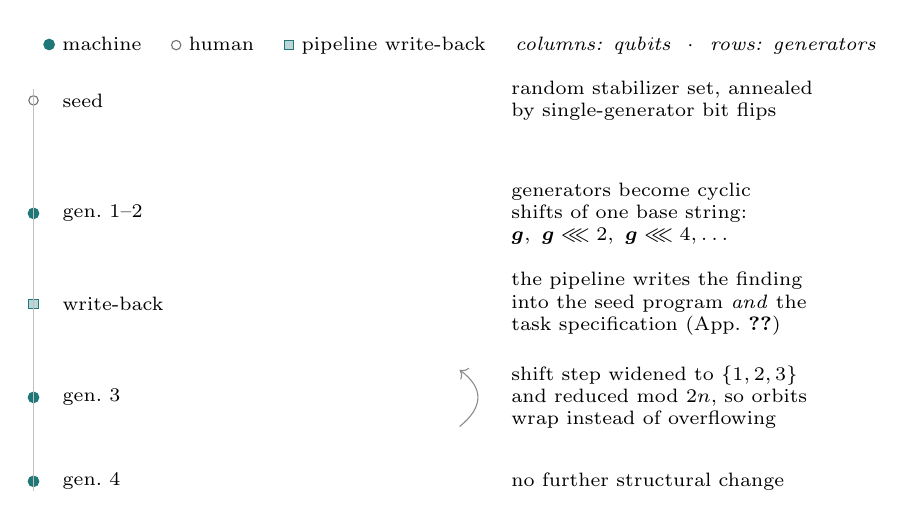
\begin{tikzpicture}[x=2.05mm, y=2.05mm, font=\scriptsize,
  lbl/.style={anchor=west, font=\scriptsize},
  ann/.style={anchor=west, font=\scriptsize, text width=40mm},
  mach/.style={circle, fill=achieve, draw=achieve, inner sep=1.35pt},
  hum/.style={circle, fill=white, draw=black!55, inner sep=1.2pt},
  pipe/.style={rectangle, fill=achieve!30, draw=achieve, inner sep=1.7pt}]

\node[anchor=west, font=\scriptsize] at (-14,3.4)
  {\tikz\node[mach]{};\ machine \quad \tikz\node[hum]{};\ human \quad
   \tikz\node[pipe]{};\ pipeline write-back \quad
   \textit{columns: qubits \ $\cdot$ \ rows: generators}};

% ---------------- seed --------------------------------------------------
\node[hum] at (-14,0) {};
\node[lbl] at (-12.8,0) {seed};
\begin{scope}[shift={(0,1.4)}]
  \foreach \r/\cs in {0/{1,4,5,9}, 1/{0,3,7}, 2/{2,5,6,10}, 3/{1,8,9,11}}
    \foreach \c in \cs { \gcell{\c}{\r}{black!30} }
\end{scope}
\node[ann] at (15,0) {random stabilizer set, annealed by single-generator
  bit flips};

% ---------------- gen 1-2: cyclic, step 1 -------------------------------
\node[mach] at (-14,-7) {};
\node[lbl] at (-12.8,-7) {gen.\ 1--2};
\begin{scope}[shift={(0,-5.6)}]
  \foreach \r in {0,1,2,3} {
    \pgfmathtruncatemacro{\a}{\r} \pgfmathtruncatemacro{\b}{\r+1}
    \pgfmathtruncatemacro{\e}{\r+4}
    \gcell{\a}{\r}{achieve} \gcell{\b}{\r}{achieve}
    \gcell{\e}{\r}{achieve!45}
  }
\end{scope}
\node[ann] at (15,-7) {generators become cyclic shifts of one base
  string: \mbox{$\vct{g},\ \vct{g}\lll 2,\ \vct{g}\lll 4,\dots$}};

% ---------------- reseed -------------------------------------------------
\node[pipe] at (-14,-12.6) {};
\node[lbl] at (-12.8,-12.6) {write-back};
\node[ann] at (15,-12.6) {the pipeline writes the finding into the seed
  program \emph{and} the task specification (App.~\ref{app:prompts})};

% ---------------- gen 3: quasi-cyclic, step 2, wrapping -----------------
\node[mach] at (-14,-18.4) {};
\node[lbl] at (-12.8,-18.4) {gen.\ 3};
\begin{scope}[shift={(0,-17)}]
  \foreach \r in {0,1,2,3} {
    \pgfmathtruncatemacro{\a}{mod(2*\r,12)}
    \pgfmathtruncatemacro{\b}{mod(2*\r+1,12)}
    \pgfmathtruncatemacro{\e}{mod(2*\r+6,12)}
    \gcell{\a}{\r}{achieve} \gcell{\b}{\r}{achieve}
    \gcell{\e}{\r}{achieve!45}
  }
  \draw[black!45, ->] (12.4,-3.2) .. controls (13.9,-2.0) and (13.9,-0.8) ..
        (12.4,0.3);
\end{scope}
\node[ann] at (15,-18.4) {shift step widened to $\{1,2,3\}$ and reduced
  $\bmod\ 2n$, so orbits wrap instead of overflowing};

% ---------------- gen 4 --------------------------------------------------
\node[mach] at (-14,-23.6) {};
\node[lbl] at (-12.8,-23.6) {gen.\ 4};
\node[ann] at (15,-23.6) {no further structural change};

\draw[black!25, line width=0.6pt] (-14,0.7) -- (-14,-24.2);
\end{tikzpicture}
\caption{Evolution of the search program.}
\label{fig:lineage}
\end{figure}


\subsection{Distance improvements}\label{sec:distance-results}

For listed cells, the tables give the July 2026 distance interval within
the previous code parameters and our verified distance in Ours $d$
(2026). Bold entries attain the applicable archived, EA-Plotkin or
certified upper bound (Section~\ref{sec:optimality-results}). References
identify previous lower-bound constructions and their dates. For
$q=4,5$, where no comparable dated entry is archived, full constructed
parameters appear in a separate \emph{New constructions} block.
No historical interval is assigned where no comparison entry exists.

% Separate numbered tables, top-aligned side by side.
\begin{table}[!ht]
\centering
\setlength{\tabcolsep}{3pt}
\renewcommand{\arraystretch}{1.18}
\begin{minipage}[t]{0.485\linewidth}
\vspace{0pt}
\centering
\footnotesize
\caption{Qubit EAQECCs ($q=2$).}
\label{tab:results}
\begin{tabular}{@{}lcc@{}}
\toprule
Previous & Ours $d$ & \multirow{2}{*}{References} \\
$[[n,k,d_\ell\text{--}d_u;c]]_q$ & (2026) & \\
\midrule
$[[7,1,5\text{--}6;4]]_2$ & $\mathbf{6}$ & \citet{GHW2020} \\
$[[9,1,7\text{--}8;6]]_2$ & $\mathbf{8}$ & \citet{Luo2022} \\
$[[10,1,7\text{--}9;6]]_2$ & $\mathbf{9}$ & \citet{Luo2022} \\
$[[11,1,9\text{--}10;8]]_2$ & $\mathbf{10}$ & \citet{Luo2022} \\
$[[12,1,9\text{--}11;8]]_2$ & $\mathbf{11}$ & \citet{Luo2022} \\
$[[12,2,7\text{--}10;9]]_2$ & $\mathbf{9}$ & \citet{Luo2022} \\
$[[13,1,9\text{--}12;8]]_2$ & $\mathbf{11}$ & \citet{Luo2022} \\
$[[13,1,11\text{--}12;10]]_2$ & $\mathbf{12}^{\dagger}$ & \citet{Luo2022} \\
$[[15,1,13\text{--}14;12]]_2$ & $\mathbf{14}^{\dagger}$ & \citet{Luo2022} \\
\bottomrule
\end{tabular}
\par\vspace{2pt}
{\scriptsize $\dagger$ Constructed by the evolved program at unseen code lengths.}
\end{minipage}\hfill
\begin{minipage}[t]{0.485\linewidth}
\vspace{0pt}
\centering
\footnotesize
\caption{Qudit EAQECCs ($q=3,4,5$).}
\label{tab:results-qudit}
\begin{tabular}{@{}lcc@{}}
\toprule
Previous & Ours $d$ & \multirow{2}{*}{References} \\
$[[n,k,d_\ell\text{--}d_u;c]]_q$ & (2026) & \\
\midrule
$[[9,1,7\text{--}8;4]]_3$ & $\mathbf{8}$ & \citet{Luo2022} \\
$[[10,1,8\text{--}9;5]]_3$ & $\mathbf{9}$ & \citet{Luo2022} \\
$[[11,1,9\text{--}10;7]]_3$ & $\mathbf{10}$ & \citet{Luo2022} \\
$[[13,1,10\text{--}12;8]]_3$ & $\mathbf{12}$ & \citet{Luo2022} \\
\midrule
\multicolumn{3}{@{}l@{}}{\emph{New constructions:} $[[n,k,d;c]]_q$} \\
\midrule
$[[10,1,9;4]]_4$ & $9$ & Ours \\
$[[12,1,11;6]]_4$ & $11$ & Ours \\
$[[14,1,13;8]]_4$ & $13$ & Ours \\
\midrule
$[[12,1,11;5]]_5$ & $11$ & Ours \\
$[[14,1,13;7]]_5$ & $13$ & Ours \\
\bottomrule
\end{tabular}
\end{minipage}
\end{table}


The tables report codes obtained across discovery campaigns, family
constructions and solver refinement. Section~\ref{sec:ablation} separately
evaluates the programs generated in the controlled study.
The daggered $n=13,15$ results show that the evolved program also
constructs codes at lengths not used for training or selection (Section~\ref{sec:longer-codes}). The $n=15$ row adds a finite construction to the table;
these parameters are already covered by the family theorem and are not
counted again among its 54 gap closures.

Our codes and the upper bounds close all nine listed qubit gaps
in Table~\ref{tab:results}. At $(n,k,c)=(10,1,6)$ and $(12,1,8)$,
the distance increases by two. Five odd-length family instances also
close listed gaps and are included in the family count below. The two
remaining qubit cells are settled by solver refinement
(Section~\ref{sec:optimality-results}). Table~\ref{tab:results-qudit}
shows four qutrit gap closures, including $[[13,1,12;8]]_3$, which raises
the listed distance from 10 to 12 at fixed length and entanglement.

The previous $[[7,1,5;4]]_2$ construction follows from the pure
$[[11,1,5]]_2$ code of \citet{CRSS1997} and the length-reduction rule of
\citet{GHW2020}; we date this EAQECC construction by the 2020 rule.
The other eight qubit baselines and the four displayed qutrit baselines
follow from the 2022 version of \citet{Luo2022}. Appendix~\ref{app:bound-history}
records the source codes and propagation rules for each cell.

The 65 core qubit code records cover 61 distinct $(n,k,c)$ cells: eight listed
and 53 absent cells. The 27 qutrit codes comprise 15 improvements
to listed entries, 11 constructions at absent cells and one code whose
distance is already listed. Multiple codes at one cell are not
counted as separate table entries. Four of these listed core cells overlap the
family results in Section~\ref{sec:family-results}. The additional
$n=15$ code record is kept in the controlled-study archive, separately from
these core-file counts.

\subsection{Code families and reduced entanglement}\label{sec:family-results}

Theorem~\ref{thm:unified} gives $[[n,1,n-1;n-q-1]]_q$ codes for
$q\ge3$ and $n\ge2q+1$, and for $q=2$ at odd $n\ge5$.
The proof establishes the entire family; the auditor checks finite
instances at $q=2,3,4,5$. The qubit instances close 29 listed gaps.
At $q=3$, increasing the supplied entanglement by one pair gives codes
at $c=n-3$, closing another 25 listed gaps. Together, these constructions
settle 54 listed entries in the archived tables.

Additional constructions attain $d=n-1$ at $c=n-q-2$.
The displayed $q=4,5$ examples include $[[10,1,9;4]]_4$ and
$[[12,1,11;5]]_5$, requiring four and five shared pairs, respectively.
These constructions establish achievable
entanglement costs; smaller costs at $q=4,5$ have not been excluded.
The archive contains 13 codes at $q=4$ and 10 at $q=5$.
Table~\ref{tab:results-qudit} selects those using the least entanglement
reached at the displayed lengths.

% GENERATED by scripts/make_bound_map_figure.py from artifacts/tables/bound_map.json
% — do not edit; re-run the script instead.
\begin{figure}[!ht]
\centering
\resizebox{0.80\linewidth}{!}{%
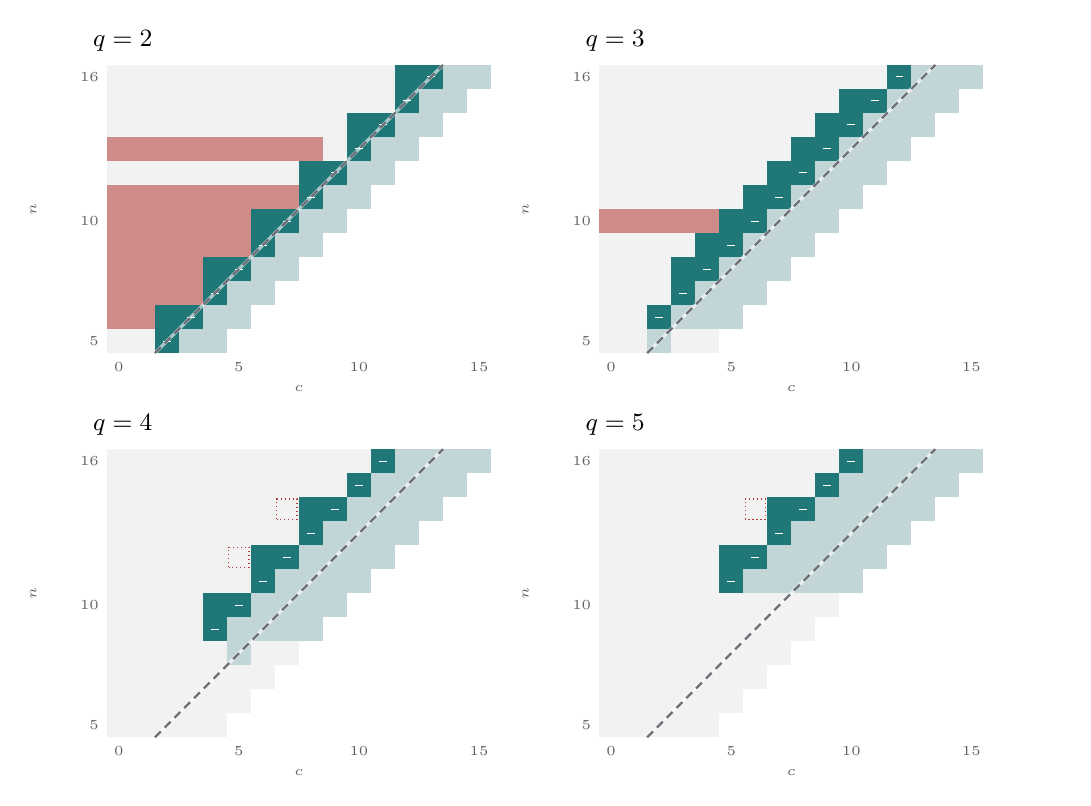
\begin{tikzpicture}[x=3.05mm, y=3.05mm, line width=0.3pt,
    ax/.style={font=\tiny, inner sep=1pt, text=black!62},
    hd/.style={font=\small, inner sep=1pt},
    lg/.style={font=\scriptsize, inner sep=1pt}]

  % ---------------- q = 2
  \begin{scope}[shift={(0.0,-0.0)}]
    \foreach \n in {5,...,16} {
      \pgfmathtruncatemacro{\cm}{min(\n-1,15)}
      \fill[black!5] (-0.5,\n-0.5) rectangle (\cm+0.5,\n+0.5);
    }
    \fill[achieve, opacity=1] (1.5,4.5) rectangle (2.5,5.5);
    \draw[white, line width=0.35pt] (1.84,5) -- (2.16,5);
    \fill[achieve, opacity=0.22] (2.5,4.5) rectangle (3.5,5.5);
    \fill[achieve, opacity=0.22] (3.5,4.5) rectangle (4.5,5.5);
    \fill[refute, opacity=0.55] (-0.5,5.5) rectangle (0.5,6.5);
    \fill[refute, opacity=0.55] (0.5,5.5) rectangle (1.5,6.5);
    \fill[achieve, opacity=1] (1.5,5.5) rectangle (2.5,6.5);
    \fill[achieve, opacity=1] (2.5,5.5) rectangle (3.5,6.5);
    \draw[white, line width=0.35pt] (2.84,6) -- (3.16,6);
    \fill[achieve, opacity=0.22] (3.5,5.5) rectangle (4.5,6.5);
    \fill[achieve, opacity=0.22] (4.5,5.5) rectangle (5.5,6.5);
    \fill[refute, opacity=0.55] (-0.5,6.5) rectangle (0.5,7.5);
    \fill[refute, opacity=0.55] (0.5,6.5) rectangle (1.5,7.5);
    \fill[refute, opacity=0.55] (1.5,6.5) rectangle (2.5,7.5);
    \fill[refute, opacity=0.55] (2.5,6.5) rectangle (3.5,7.5);
    \fill[achieve, opacity=1] (3.5,6.5) rectangle (4.5,7.5);
    \draw[white, line width=0.35pt] (3.84,7) -- (4.16,7);
    \fill[achieve, opacity=0.22] (4.5,6.5) rectangle (5.5,7.5);
    \fill[achieve, opacity=0.22] (5.5,6.5) rectangle (6.5,7.5);
    \fill[refute, opacity=0.55] (-0.5,7.5) rectangle (0.5,8.5);
    \fill[refute, opacity=0.55] (0.5,7.5) rectangle (1.5,8.5);
    \fill[refute, opacity=0.55] (1.5,7.5) rectangle (2.5,8.5);
    \fill[refute, opacity=0.55] (2.5,7.5) rectangle (3.5,8.5);
    \fill[achieve, opacity=1] (3.5,7.5) rectangle (4.5,8.5);
    \fill[achieve, opacity=1] (4.5,7.5) rectangle (5.5,8.5);
    \draw[white, line width=0.35pt] (4.84,8) -- (5.16,8);
    \fill[achieve, opacity=0.22] (5.5,7.5) rectangle (6.5,8.5);
    \fill[achieve, opacity=0.22] (6.5,7.5) rectangle (7.5,8.5);
    \fill[refute, opacity=0.55] (-0.5,8.5) rectangle (0.5,9.5);
    \fill[refute, opacity=0.55] (0.5,8.5) rectangle (1.5,9.5);
    \fill[refute, opacity=0.55] (1.5,8.5) rectangle (2.5,9.5);
    \fill[refute, opacity=0.55] (2.5,8.5) rectangle (3.5,9.5);
    \fill[refute, opacity=0.55] (3.5,8.5) rectangle (4.5,9.5);
    \fill[refute, opacity=0.55] (4.5,8.5) rectangle (5.5,9.5);
    \fill[achieve, opacity=1] (5.5,8.5) rectangle (6.5,9.5);
    \draw[white, line width=0.35pt] (5.84,9) -- (6.16,9);
    \fill[achieve, opacity=0.22] (6.5,8.5) rectangle (7.5,9.5);
    \fill[achieve, opacity=0.22] (7.5,8.5) rectangle (8.5,9.5);
    \fill[refute, opacity=0.55] (-0.5,9.5) rectangle (0.5,10.5);
    \fill[refute, opacity=0.55] (0.5,9.5) rectangle (1.5,10.5);
    \fill[refute, opacity=0.55] (1.5,9.5) rectangle (2.5,10.5);
    \fill[refute, opacity=0.55] (2.5,9.5) rectangle (3.5,10.5);
    \fill[refute, opacity=0.55] (3.5,9.5) rectangle (4.5,10.5);
    \fill[refute, opacity=0.55] (4.5,9.5) rectangle (5.5,10.5);
    \fill[achieve, opacity=1] (5.5,9.5) rectangle (6.5,10.5);
    \fill[achieve, opacity=1] (6.5,9.5) rectangle (7.5,10.5);
    \draw[white, line width=0.35pt] (6.84,10) -- (7.16,10);
    \fill[achieve, opacity=0.22] (7.5,9.5) rectangle (8.5,10.5);
    \fill[achieve, opacity=0.22] (8.5,9.5) rectangle (9.5,10.5);
    \fill[refute, opacity=0.55] (-0.5,10.5) rectangle (0.5,11.5);
    \fill[refute, opacity=0.55] (0.5,10.5) rectangle (1.5,11.5);
    \fill[refute, opacity=0.55] (1.5,10.5) rectangle (2.5,11.5);
    \fill[refute, opacity=0.55] (2.5,10.5) rectangle (3.5,11.5);
    \fill[refute, opacity=0.55] (3.5,10.5) rectangle (4.5,11.5);
    \fill[refute, opacity=0.55] (4.5,10.5) rectangle (5.5,11.5);
    \fill[refute, opacity=0.55] (5.5,10.5) rectangle (6.5,11.5);
    \fill[refute, opacity=0.55] (6.5,10.5) rectangle (7.5,11.5);
    \fill[achieve, opacity=1] (7.5,10.5) rectangle (8.5,11.5);
    \draw[white, line width=0.35pt] (7.84,11) -- (8.16,11);
    \fill[achieve, opacity=0.22] (8.5,10.5) rectangle (9.5,11.5);
    \fill[achieve, opacity=0.22] (9.5,10.5) rectangle (10.5,11.5);
    \fill[achieve, opacity=1] (7.5,11.5) rectangle (8.5,12.5);
    \fill[achieve, opacity=1] (8.5,11.5) rectangle (9.5,12.5);
    \draw[white, line width=0.35pt] (8.84,12) -- (9.16,12);
    \fill[achieve, opacity=0.22] (9.5,11.5) rectangle (10.5,12.5);
    \fill[achieve, opacity=0.22] (10.5,11.5) rectangle (11.5,12.5);
    \fill[refute, opacity=0.55] (-0.5,12.5) rectangle (0.5,13.5);
    \fill[refute, opacity=0.55] (0.5,12.5) rectangle (1.5,13.5);
    \fill[refute, opacity=0.55] (1.5,12.5) rectangle (2.5,13.5);
    \fill[refute, opacity=0.55] (2.5,12.5) rectangle (3.5,13.5);
    \fill[refute, opacity=0.55] (3.5,12.5) rectangle (4.5,13.5);
    \fill[refute, opacity=0.55] (4.5,12.5) rectangle (5.5,13.5);
    \fill[refute, opacity=0.55] (5.5,12.5) rectangle (6.5,13.5);
    \fill[refute, opacity=0.55] (6.5,12.5) rectangle (7.5,13.5);
    \fill[refute, opacity=0.55] (7.5,12.5) rectangle (8.5,13.5);
    \fill[achieve, opacity=1] (9.5,12.5) rectangle (10.5,13.5);
    \draw[white, line width=0.35pt] (9.84,13) -- (10.16,13);
    \fill[achieve, opacity=0.22] (10.5,12.5) rectangle (11.5,13.5);
    \fill[achieve, opacity=0.22] (11.5,12.5) rectangle (12.5,13.5);
    \fill[achieve, opacity=1] (9.5,13.5) rectangle (10.5,14.5);
    \fill[achieve, opacity=1] (10.5,13.5) rectangle (11.5,14.5);
    \draw[white, line width=0.35pt] (10.84,14) -- (11.16,14);
    \fill[achieve, opacity=0.22] (11.5,13.5) rectangle (12.5,14.5);
    \fill[achieve, opacity=0.22] (12.5,13.5) rectangle (13.5,14.5);
    \fill[achieve, opacity=1] (11.5,14.5) rectangle (12.5,15.5);
    \draw[white, line width=0.35pt] (11.84,15) -- (12.16,15);
    \fill[achieve, opacity=0.22] (12.5,14.5) rectangle (13.5,15.5);
    \fill[achieve, opacity=0.22] (13.5,14.5) rectangle (14.5,15.5);
    \fill[achieve, opacity=1] (11.5,15.5) rectangle (12.5,16.5);
    \fill[achieve, opacity=1] (12.5,15.5) rectangle (13.5,16.5);
    \draw[white, line width=0.35pt] (12.84,16) -- (13.16,16);
    \fill[achieve, opacity=0.22] (13.5,15.5) rectangle (14.5,16.5);
    \fill[achieve, opacity=0.22] (14.5,15.5) rectangle (15.5,16.5);
    \draw[white, opacity=0.6, line width=1.2pt] (1.5,4.5) -- (13.5,16.5);
    \draw[bdh, line width=0.8pt, densely dashed] (1.5,4.5) -- (13.5,16.5);
    \node[ax, anchor=east] at (-0.7,5) {$5$};
    \node[ax, anchor=east] at (-0.7,10) {$10$};
    \node[ax, anchor=east] at (-0.7,16) {$16$};
    \node[ax, anchor=south, rotate=90] at (-3.3,10.5) {$n$};
    \node[ax, anchor=north] at (0,4.25) {$0$};
    \node[ax, anchor=north] at (5,4.25) {$5$};
    \node[ax, anchor=north] at (10,4.25) {$10$};
    \node[ax, anchor=north] at (15,4.25) {$15$};
    \node[ax, anchor=north] at (7.5,3.3) {$c$};
    \node[hd, anchor=west] at (-1.2,17.5) {$q=2$};
  \end{scope}

  % ---------------- q = 3
  \begin{scope}[shift={(20.5,-0.0)}]
    \foreach \n in {5,...,16} {
      \pgfmathtruncatemacro{\cm}{min(\n-1,15)}
      \fill[black!5] (-0.5,\n-0.5) rectangle (\cm+0.5,\n+0.5);
    }
    \fill[achieve, opacity=0.22] (1.5,4.5) rectangle (2.5,5.5);
    \fill[achieve, opacity=1] (1.5,5.5) rectangle (2.5,6.5);
    \draw[white, line width=0.35pt] (1.84,6) -- (2.16,6);
    \fill[achieve, opacity=0.22] (2.5,5.5) rectangle (3.5,6.5);
    \fill[achieve, opacity=0.22] (3.5,5.5) rectangle (4.5,6.5);
    \fill[achieve, opacity=0.22] (4.5,5.5) rectangle (5.5,6.5);
    \fill[achieve, opacity=1] (2.5,6.5) rectangle (3.5,7.5);
    \draw[white, line width=0.35pt] (2.84,7) -- (3.16,7);
    \fill[achieve, opacity=0.22] (3.5,6.5) rectangle (4.5,7.5);
    \fill[achieve, opacity=0.22] (4.5,6.5) rectangle (5.5,7.5);
    \fill[achieve, opacity=0.22] (5.5,6.5) rectangle (6.5,7.5);
    \fill[achieve, opacity=1] (2.5,7.5) rectangle (3.5,8.5);
    \fill[achieve, opacity=1] (3.5,7.5) rectangle (4.5,8.5);
    \draw[white, line width=0.35pt] (3.84,8) -- (4.16,8);
    \fill[achieve, opacity=0.22] (4.5,7.5) rectangle (5.5,8.5);
    \fill[achieve, opacity=0.22] (5.5,7.5) rectangle (6.5,8.5);
    \fill[achieve, opacity=0.22] (6.5,7.5) rectangle (7.5,8.5);
    \fill[achieve, opacity=1] (3.5,8.5) rectangle (4.5,9.5);
    \fill[achieve, opacity=1] (4.5,8.5) rectangle (5.5,9.5);
    \draw[white, line width=0.35pt] (4.84,9) -- (5.16,9);
    \fill[achieve, opacity=0.22] (5.5,8.5) rectangle (6.5,9.5);
    \fill[achieve, opacity=0.22] (6.5,8.5) rectangle (7.5,9.5);
    \fill[achieve, opacity=0.22] (7.5,8.5) rectangle (8.5,9.5);
    \fill[refute, opacity=0.55] (-0.5,9.5) rectangle (0.5,10.5);
    \fill[refute, opacity=0.55] (0.5,9.5) rectangle (1.5,10.5);
    \fill[refute, opacity=0.55] (1.5,9.5) rectangle (2.5,10.5);
    \fill[refute, opacity=0.55] (2.5,9.5) rectangle (3.5,10.5);
    \fill[refute, opacity=0.55] (3.5,9.5) rectangle (4.5,10.5);
    \fill[achieve, opacity=1] (4.5,9.5) rectangle (5.5,10.5);
    \fill[achieve, opacity=1] (5.5,9.5) rectangle (6.5,10.5);
    \draw[white, line width=0.35pt] (5.84,10) -- (6.16,10);
    \fill[achieve, opacity=0.22] (6.5,9.5) rectangle (7.5,10.5);
    \fill[achieve, opacity=0.22] (7.5,9.5) rectangle (8.5,10.5);
    \fill[achieve, opacity=0.22] (8.5,9.5) rectangle (9.5,10.5);
    \fill[achieve, opacity=1] (5.5,10.5) rectangle (6.5,11.5);
    \fill[achieve, opacity=1] (6.5,10.5) rectangle (7.5,11.5);
    \draw[white, line width=0.35pt] (6.84,11) -- (7.16,11);
    \fill[achieve, opacity=0.22] (7.5,10.5) rectangle (8.5,11.5);
    \fill[achieve, opacity=0.22] (8.5,10.5) rectangle (9.5,11.5);
    \fill[achieve, opacity=0.22] (9.5,10.5) rectangle (10.5,11.5);
    \fill[achieve, opacity=1] (6.5,11.5) rectangle (7.5,12.5);
    \fill[achieve, opacity=1] (7.5,11.5) rectangle (8.5,12.5);
    \draw[white, line width=0.35pt] (7.84,12) -- (8.16,12);
    \fill[achieve, opacity=0.22] (8.5,11.5) rectangle (9.5,12.5);
    \fill[achieve, opacity=0.22] (9.5,11.5) rectangle (10.5,12.5);
    \fill[achieve, opacity=0.22] (10.5,11.5) rectangle (11.5,12.5);
    \fill[achieve, opacity=1] (7.5,12.5) rectangle (8.5,13.5);
    \fill[achieve, opacity=1] (8.5,12.5) rectangle (9.5,13.5);
    \draw[white, line width=0.35pt] (8.84,13) -- (9.16,13);
    \fill[achieve, opacity=0.22] (9.5,12.5) rectangle (10.5,13.5);
    \fill[achieve, opacity=0.22] (10.5,12.5) rectangle (11.5,13.5);
    \fill[achieve, opacity=0.22] (11.5,12.5) rectangle (12.5,13.5);
    \fill[achieve, opacity=1] (8.5,13.5) rectangle (9.5,14.5);
    \fill[achieve, opacity=1] (9.5,13.5) rectangle (10.5,14.5);
    \draw[white, line width=0.35pt] (9.84,14) -- (10.16,14);
    \fill[achieve, opacity=0.22] (10.5,13.5) rectangle (11.5,14.5);
    \fill[achieve, opacity=0.22] (11.5,13.5) rectangle (12.5,14.5);
    \fill[achieve, opacity=0.22] (12.5,13.5) rectangle (13.5,14.5);
    \fill[achieve, opacity=1] (9.5,14.5) rectangle (10.5,15.5);
    \fill[achieve, opacity=1] (10.5,14.5) rectangle (11.5,15.5);
    \draw[white, line width=0.35pt] (10.84,15) -- (11.16,15);
    \fill[achieve, opacity=0.22] (11.5,14.5) rectangle (12.5,15.5);
    \fill[achieve, opacity=0.22] (12.5,14.5) rectangle (13.5,15.5);
    \fill[achieve, opacity=0.22] (13.5,14.5) rectangle (14.5,15.5);
    \fill[achieve, opacity=1] (11.5,15.5) rectangle (12.5,16.5);
    \draw[white, line width=0.35pt] (11.84,16) -- (12.16,16);
    \fill[achieve, opacity=0.22] (12.5,15.5) rectangle (13.5,16.5);
    \fill[achieve, opacity=0.22] (13.5,15.5) rectangle (14.5,16.5);
    \fill[achieve, opacity=0.22] (14.5,15.5) rectangle (15.5,16.5);
    \draw[white, opacity=0.6, line width=1.2pt] (1.5,4.5) -- (13.5,16.5);
    \draw[bdh, line width=0.8pt, densely dashed] (1.5,4.5) -- (13.5,16.5);
    \node[ax, anchor=east] at (-0.7,5) {$5$};
    \node[ax, anchor=east] at (-0.7,10) {$10$};
    \node[ax, anchor=east] at (-0.7,16) {$16$};
    \node[ax, anchor=south, rotate=90] at (-3.3,10.5) {$n$};
    \node[ax, anchor=north] at (0,4.25) {$0$};
    \node[ax, anchor=north] at (5,4.25) {$5$};
    \node[ax, anchor=north] at (10,4.25) {$10$};
    \node[ax, anchor=north] at (15,4.25) {$15$};
    \node[ax, anchor=north] at (7.5,3.3) {$c$};
    \node[hd, anchor=west] at (-1.2,17.5) {$q=3$};
  \end{scope}

  % ---------------- q = 4
  \begin{scope}[shift={(0.0,-16.0)}]
    \foreach \n in {5,...,16} {
      \pgfmathtruncatemacro{\cm}{min(\n-1,15)}
      \fill[black!5] (-0.5,\n-0.5) rectangle (\cm+0.5,\n+0.5);
    }
    \fill[achieve, opacity=0.22] (4.5,7.5) rectangle (5.5,8.5);
    \fill[achieve, opacity=1] (3.5,8.5) rectangle (4.5,9.5);
    \draw[white, line width=0.35pt] (3.84,9) -- (4.16,9);
    \fill[achieve, opacity=0.22] (4.5,8.5) rectangle (5.5,9.5);
    \fill[achieve, opacity=0.22] (5.5,8.5) rectangle (6.5,9.5);
    \fill[achieve, opacity=0.22] (6.5,8.5) rectangle (7.5,9.5);
    \fill[achieve, opacity=0.22] (7.5,8.5) rectangle (8.5,9.5);
    \fill[achieve, opacity=1] (3.5,9.5) rectangle (4.5,10.5);
    \fill[achieve, opacity=1] (4.5,9.5) rectangle (5.5,10.5);
    \draw[white, line width=0.35pt] (4.84,10) -- (5.16,10);
    \fill[achieve, opacity=0.22] (5.5,9.5) rectangle (6.5,10.5);
    \fill[achieve, opacity=0.22] (6.5,9.5) rectangle (7.5,10.5);
    \fill[achieve, opacity=0.22] (7.5,9.5) rectangle (8.5,10.5);
    \fill[achieve, opacity=0.22] (8.5,9.5) rectangle (9.5,10.5);
    \fill[achieve, opacity=1] (5.5,10.5) rectangle (6.5,11.5);
    \draw[white, line width=0.35pt] (5.84,11) -- (6.16,11);
    \fill[achieve, opacity=0.22] (6.5,10.5) rectangle (7.5,11.5);
    \fill[achieve, opacity=0.22] (7.5,10.5) rectangle (8.5,11.5);
    \fill[achieve, opacity=0.22] (8.5,10.5) rectangle (9.5,11.5);
    \fill[achieve, opacity=0.22] (9.5,10.5) rectangle (10.5,11.5);
    \draw[refute, line width=0.45pt, densely dotted] (4.58,11.58) rectangle (5.42,12.42);
    \fill[achieve, opacity=1] (5.5,11.5) rectangle (6.5,12.5);
    \fill[achieve, opacity=1] (6.5,11.5) rectangle (7.5,12.5);
    \draw[white, line width=0.35pt] (6.84,12) -- (7.16,12);
    \fill[achieve, opacity=0.22] (7.5,11.5) rectangle (8.5,12.5);
    \fill[achieve, opacity=0.22] (8.5,11.5) rectangle (9.5,12.5);
    \fill[achieve, opacity=0.22] (9.5,11.5) rectangle (10.5,12.5);
    \fill[achieve, opacity=0.22] (10.5,11.5) rectangle (11.5,12.5);
    \fill[achieve, opacity=1] (7.5,12.5) rectangle (8.5,13.5);
    \draw[white, line width=0.35pt] (7.84,13) -- (8.16,13);
    \fill[achieve, opacity=0.22] (8.5,12.5) rectangle (9.5,13.5);
    \fill[achieve, opacity=0.22] (9.5,12.5) rectangle (10.5,13.5);
    \fill[achieve, opacity=0.22] (10.5,12.5) rectangle (11.5,13.5);
    \fill[achieve, opacity=0.22] (11.5,12.5) rectangle (12.5,13.5);
    \draw[refute, line width=0.45pt, densely dotted] (6.58,13.58) rectangle (7.42,14.42);
    \fill[achieve, opacity=1] (7.5,13.5) rectangle (8.5,14.5);
    \fill[achieve, opacity=1] (8.5,13.5) rectangle (9.5,14.5);
    \draw[white, line width=0.35pt] (8.84,14) -- (9.16,14);
    \fill[achieve, opacity=0.22] (9.5,13.5) rectangle (10.5,14.5);
    \fill[achieve, opacity=0.22] (10.5,13.5) rectangle (11.5,14.5);
    \fill[achieve, opacity=0.22] (11.5,13.5) rectangle (12.5,14.5);
    \fill[achieve, opacity=0.22] (12.5,13.5) rectangle (13.5,14.5);
    \fill[achieve, opacity=1] (9.5,14.5) rectangle (10.5,15.5);
    \draw[white, line width=0.35pt] (9.84,15) -- (10.16,15);
    \fill[achieve, opacity=0.22] (10.5,14.5) rectangle (11.5,15.5);
    \fill[achieve, opacity=0.22] (11.5,14.5) rectangle (12.5,15.5);
    \fill[achieve, opacity=0.22] (12.5,14.5) rectangle (13.5,15.5);
    \fill[achieve, opacity=0.22] (13.5,14.5) rectangle (14.5,15.5);
    \fill[achieve, opacity=1] (10.5,15.5) rectangle (11.5,16.5);
    \draw[white, line width=0.35pt] (10.84,16) -- (11.16,16);
    \fill[achieve, opacity=0.22] (11.5,15.5) rectangle (12.5,16.5);
    \fill[achieve, opacity=0.22] (12.5,15.5) rectangle (13.5,16.5);
    \fill[achieve, opacity=0.22] (13.5,15.5) rectangle (14.5,16.5);
    \fill[achieve, opacity=0.22] (14.5,15.5) rectangle (15.5,16.5);
    \draw[white, opacity=0.6, line width=1.2pt] (1.5,4.5) -- (13.5,16.5);
    \draw[bdh, line width=0.8pt, densely dashed] (1.5,4.5) -- (13.5,16.5);
    \node[ax, anchor=east] at (-0.7,5) {$5$};
    \node[ax, anchor=east] at (-0.7,10) {$10$};
    \node[ax, anchor=east] at (-0.7,16) {$16$};
    \node[ax, anchor=south, rotate=90] at (-3.3,10.5) {$n$};
    \node[ax, anchor=north] at (0,4.25) {$0$};
    \node[ax, anchor=north] at (5,4.25) {$5$};
    \node[ax, anchor=north] at (10,4.25) {$10$};
    \node[ax, anchor=north] at (15,4.25) {$15$};
    \node[ax, anchor=north] at (7.5,3.3) {$c$};
    \node[hd, anchor=west] at (-1.2,17.5) {$q=4$};
  \end{scope}

  % ---------------- q = 5
  \begin{scope}[shift={(20.5,-16.0)}]
    \foreach \n in {5,...,16} {
      \pgfmathtruncatemacro{\cm}{min(\n-1,15)}
      \fill[black!5] (-0.5,\n-0.5) rectangle (\cm+0.5,\n+0.5);
    }
    \fill[achieve, opacity=1] (4.5,10.5) rectangle (5.5,11.5);
    \draw[white, line width=0.35pt] (4.84,11) -- (5.16,11);
    \fill[achieve, opacity=0.22] (5.5,10.5) rectangle (6.5,11.5);
    \fill[achieve, opacity=0.22] (6.5,10.5) rectangle (7.5,11.5);
    \fill[achieve, opacity=0.22] (7.5,10.5) rectangle (8.5,11.5);
    \fill[achieve, opacity=0.22] (8.5,10.5) rectangle (9.5,11.5);
    \fill[achieve, opacity=0.22] (9.5,10.5) rectangle (10.5,11.5);
    \fill[achieve, opacity=1] (4.5,11.5) rectangle (5.5,12.5);
    \fill[achieve, opacity=1] (5.5,11.5) rectangle (6.5,12.5);
    \draw[white, line width=0.35pt] (5.84,12) -- (6.16,12);
    \fill[achieve, opacity=0.22] (6.5,11.5) rectangle (7.5,12.5);
    \fill[achieve, opacity=0.22] (7.5,11.5) rectangle (8.5,12.5);
    \fill[achieve, opacity=0.22] (8.5,11.5) rectangle (9.5,12.5);
    \fill[achieve, opacity=0.22] (9.5,11.5) rectangle (10.5,12.5);
    \fill[achieve, opacity=0.22] (10.5,11.5) rectangle (11.5,12.5);
    \fill[achieve, opacity=1] (6.5,12.5) rectangle (7.5,13.5);
    \draw[white, line width=0.35pt] (6.84,13) -- (7.16,13);
    \fill[achieve, opacity=0.22] (7.5,12.5) rectangle (8.5,13.5);
    \fill[achieve, opacity=0.22] (8.5,12.5) rectangle (9.5,13.5);
    \fill[achieve, opacity=0.22] (9.5,12.5) rectangle (10.5,13.5);
    \fill[achieve, opacity=0.22] (10.5,12.5) rectangle (11.5,13.5);
    \fill[achieve, opacity=0.22] (11.5,12.5) rectangle (12.5,13.5);
    \draw[refute, line width=0.45pt, densely dotted] (5.58,13.58) rectangle (6.42,14.42);
    \fill[achieve, opacity=1] (6.5,13.5) rectangle (7.5,14.5);
    \fill[achieve, opacity=1] (7.5,13.5) rectangle (8.5,14.5);
    \draw[white, line width=0.35pt] (7.84,14) -- (8.16,14);
    \fill[achieve, opacity=0.22] (8.5,13.5) rectangle (9.5,14.5);
    \fill[achieve, opacity=0.22] (9.5,13.5) rectangle (10.5,14.5);
    \fill[achieve, opacity=0.22] (10.5,13.5) rectangle (11.5,14.5);
    \fill[achieve, opacity=0.22] (11.5,13.5) rectangle (12.5,14.5);
    \fill[achieve, opacity=0.22] (12.5,13.5) rectangle (13.5,14.5);
    \fill[achieve, opacity=1] (8.5,14.5) rectangle (9.5,15.5);
    \draw[white, line width=0.35pt] (8.84,15) -- (9.16,15);
    \fill[achieve, opacity=0.22] (9.5,14.5) rectangle (10.5,15.5);
    \fill[achieve, opacity=0.22] (10.5,14.5) rectangle (11.5,15.5);
    \fill[achieve, opacity=0.22] (11.5,14.5) rectangle (12.5,15.5);
    \fill[achieve, opacity=0.22] (12.5,14.5) rectangle (13.5,15.5);
    \fill[achieve, opacity=0.22] (13.5,14.5) rectangle (14.5,15.5);
    \fill[achieve, opacity=1] (9.5,15.5) rectangle (10.5,16.5);
    \draw[white, line width=0.35pt] (9.84,16) -- (10.16,16);
    \fill[achieve, opacity=0.22] (10.5,15.5) rectangle (11.5,16.5);
    \fill[achieve, opacity=0.22] (11.5,15.5) rectangle (12.5,16.5);
    \fill[achieve, opacity=0.22] (12.5,15.5) rectangle (13.5,16.5);
    \fill[achieve, opacity=0.22] (13.5,15.5) rectangle (14.5,16.5);
    \fill[achieve, opacity=0.22] (14.5,15.5) rectangle (15.5,16.5);
    \draw[white, opacity=0.6, line width=1.2pt] (1.5,4.5) -- (13.5,16.5);
    \draw[bdh, line width=0.8pt, densely dashed] (1.5,4.5) -- (13.5,16.5);
    \node[ax, anchor=east] at (-0.7,5) {$5$};
    \node[ax, anchor=east] at (-0.7,10) {$10$};
    \node[ax, anchor=east] at (-0.7,16) {$16$};
    \node[ax, anchor=south, rotate=90] at (-3.3,10.5) {$n$};
    \node[ax, anchor=north] at (0,4.25) {$0$};
    \node[ax, anchor=north] at (5,4.25) {$5$};
    \node[ax, anchor=north] at (10,4.25) {$10$};
    \node[ax, anchor=north] at (15,4.25) {$15$};
    \node[ax, anchor=north] at (7.5,3.3) {$c$};
    \node[hd, anchor=west] at (-1.2,17.5) {$q=5$};
  \end{scope}
\coordinate (panel-center) at (17.75,0);
\path let \p1=(current bounding box.south west),
          \p2=(current bounding box.north east), \p3=(panel-center)
      in ({2*\x3-\x1},\y2);
\end{tikzpicture}}\par\vspace{1.5mm}
\begingroup\footnotesize
\setlength{\tabcolsep}{3pt}\renewcommand{\arraystretch}{1.18}
\begin{tabularx}{\linewidth}{@{}lX@{\hspace{1em}}lX@{}}
\tikz[baseline=-.6ex,x=2.7mm,y=2.7mm]{\fill[achieve] (0,0) rectangle (0.9,0.9); \draw[white,line width=0.35pt] (0.3,0.45)--(0.6,0.45);} & Code exists: $c=n-q-1$ & \tikz[baseline=-.6ex,x=2.7mm,y=2.7mm]{\fill[achieve] (0,0) rectangle (0.9,0.9);} & Code exists: $c<n-q-1$\\[1pt]
\tikz[baseline=-.6ex,x=2.7mm,y=2.7mm]{\fill[achieve,opacity=0.22] (0,0) rectangle (0.9,0.9);} & Code exists: $c>n-q-1$ & \tikz[baseline=-.6ex,x=2.7mm,y=2.7mm]{\fill[refute,opacity=0.55] (0,0) rectangle (0.9,0.9);} & Nonexistence certified, including implications at smaller $c$\\[1pt]
\tikz[baseline=-.6ex,x=2.7mm,y=2.7mm]{\draw[refute,line width=0.45pt,densely dotted] (0.05,0.05) rectangle (0.85,0.85);} & Search found no witness; nonexistence unproved & \tikz[baseline=-.6ex,x=2.7mm,y=2.7mm]{\draw[bdh,line width=0.7pt,densely dashed] (0,0.45)--(0.9,0.45);} & Reference $c=n-3$; not a general bound\\[1pt]
\tikz[baseline=-.6ex]{\fill[black!5] (0,0) rectangle (2.4mm,2.4mm);} & \multicolumn{3}{l}{Unmarked gray cell: no result asserted in this figure.}
\end{tabularx}\endgroup
\caption{Linear stabilizer EAQECCs at $k=1$, target distance $n-1$.}
\label{fig:map}
\end{figure}


Figure~\ref{fig:map} concerns linear stabilizer EAQECCs with $k=1$
and target distance $n-1$. Teal at $(q,n,c)$ denotes a construction
with distance at least $n-1$. The white tick, solid fill and
pale fill distinguish $c=n-q-1$, smaller $c$ and larger $c$, respectively;
these are positions relative to the family line, not claims of minimum
entanglement. Pale cells correspond to explicit constructions or ebit
lifting. Red cells are excluded by released, checked certificates or
by their implications at smaller $c$ through ebit lifting. A dotted
outline records an unsuccessful search, not nonexistence. Unmarked gray
cells assert neither construction nor exclusion. The dashed $c=n-3$
line is the historical Brun--Devetak--Hsieh comparison, not a general
bound in this regime (Appendix~\ref{app:tables}).

\subsection{Upper bounds and optimality}\label{sec:optimality-results}

Solver refinement settles the two remaining qubit gaps from
Table~\ref{tab:results}. Normal-form SAT finds $[[12,2,9;9]]_2$,
improving our previous $d=8$ code. EA-Plotkin gives
$d\le\lfloor144/15\rfloor=9$, so the new code is distance-optimal.
At $(n,k,c)=(13,1,8)$, a DRAT-certified refutation excludes $d\ge12$;
our existing $d=11$ code is therefore optimal. Both codes are
checked by separate binary linear-algebra code, and DRAT-trim replays
the nonexistence certificate. We attribute these two closures to solver refinement.

Matching nonexistence results also establish minimum entanglement at
selected lengths. For qubits at $k=1$, $d=n-1$, the minimum is $n-3$
at $n=7,9,11$ and $n-4$ at $n=6,8,10$. For qutrits, the certified
exclusion of $[[10,1,9;4]]_3$ and a code at $c=5$ give
$\cmins(10,1,9)=5$. These exclusions have checked DRAT certificates,
with one large qubit proof regenerated on demand. Two further certified
exclusions, $[[5,2,4;3]]_2$ and $[[6,2,5;4]]_2$, were also checked by
exhaustive enumeration.

Applying the EA-Plotkin bound of \citet{GuoLi2013} additionally lowers
398 listed upper bounds. The auditor recomputes these corrections
against the reference table data. These corrections follow from a known
inequality and are reported as a separate source of upper bounds.


\FloatBarrier
%==============================================================
\section{Ablation Study}\label{sec:ablation}
%==============================================================

We test whether iterative feedback helps develop a researcher-proposed
change into an effective search program. Both policies receive the same
initial code and research guidance; their difference is how they reuse
previous programs and execution feedback.

\subsection{Program generation}
The shared proposal is to maintain and mutate a basis of
$L=S^\perp$, converting it to $S$ for exact evaluation. For
$[[9,1,8;6]]_2$ and $[[11,1,10;8]]_2$, this replaces a basis of 14 or
18 generators with four vectors. Symplectic complementation preserves
the feasible code set but changes the variables and local mutations.
A preliminary calibration compares the initial $S$-side program with
a working $L$-side control and fixes a budget at which the change can
produce measurable success. Neither the control's source nor generator
matrices are supplied to the model.

\emph{Independent proposals} always receive the initial program and its
fixed training measurements. \emph{Iterative evolution} receives the
best-so-far program and the most recent attempt, including rejected
attempts, with training feedback for both. The model can revise the
representation, objective, mutation operators and restart policy.
A proposal is a whole program revision; an evaluator call checks one
candidate matrix produced by that program. Both use Gemini 3.5 Flash
and identical tool access. There is no
controller initialization: every success must be produced by the
submitted program.

The balanced comparison contains four blocks and seven proposals per
policy and block, 56 total. Unavailable model responses interrupted the
planned 12-proposal runs; before held-out evaluation, a completion-only
rule retained the common prefix. Training uses two seeds and 10,000
exact evaluations per target. Four new validation seeds select among
each policy's three training-best distinct programs; eight further
seeds measure held-out performance. Only training feedback enters
generation. Appendix~\ref{app:ablations} records calibration, selection
and the interruption amendment.

% The plot inherits the same LaTeX Times font as Figure 2.
\begin{figure}[!ht]
\centering
\resizebox{\linewidth}{!}{% Data-derived TikZ; the main document supplies the same font as Figure 2.
\definecolor{hcinitial}{HTML}{A37545}
\definecolor{hcind}{HTML}{78818E}
\definecolor{hcevo}{HTML}{00858B}
\begin{tikzpicture}[x=1cm,y=1cm,font=\scriptsize,baseline]
\path[use as bounding box] (-1.05,-1.32) rectangle (13.15,4.35);
\begin{scope}[xshift=0cm]
\node[font=\scriptsize\bfseries] at (2.825,4.14) {(a) $n=9,\ d=8$};
\draw[black!12,line width=.35pt] (0,0.0)--(5.65,0.0);
\node[anchor=east] at (-.12,0.0) {0};
\draw[black!12,line width=.35pt] (0,0.9125)--(5.65,0.9125);
\node[anchor=east] at (-.12,0.9125) {25};
\draw[black!12,line width=.35pt] (0,1.825)--(5.65,1.825);
\node[anchor=east] at (-.12,1.825) {50};
\draw[black!12,line width=.35pt] (0,2.7375)--(5.65,2.7375);
\node[anchor=east] at (-.12,2.7375) {75};
\draw[black!12,line width=.35pt] (0,3.65)--(5.65,3.65);
\node[anchor=east] at (-.12,3.65) {100};
\draw[black!40,line width=.4pt] (0,3.65)--(0,0)--(5.65,0);
\node[rotate=90] at (-.72,1.825) {Success rate (\%)};
\node at (2.825,-.66) {Exact evaluations};
\node[anchor=north] at (0,-.12) {0};
\node[anchor=north] at (2.825,-.12) {5k};
\node[anchor=north] at (5.65,-.12) {10k};
\draw[hcind,line width=1.15pt] (0.00000,0.00000) -- (0.74241,0.00000) -- (0.74241,0.22812) -- (0.79495,0.22812) -- (0.79495,0.34219) -- (0.86332,0.34219) -- (0.86332,0.57031) -- (0.93621,0.57031) -- (0.93621,0.68437) -- (1.04582,0.68437) -- (1.04582,0.79844) -- (1.21249,0.79844) -- (1.21249,0.91250) -- (1.46166,0.91250) -- (1.46166,1.02656) -- (1.57014,1.02656) -- (1.57014,1.14062) -- (1.67975,1.14062) -- (1.67975,1.25469) -- (1.79614,1.25469) -- (1.79614,1.36875) -- (1.88993,1.36875) -- (1.88993,1.48281) -- (2.16621,1.48281) -- (2.16621,1.59688) -- (2.80071,1.59688) -- (2.80071,1.71094) -- (2.80296,1.71094) -- (2.80296,1.82500) -- (5.65000,1.82500);
\node[anchor=east,text=hcind,font=\scriptsize\bfseries] at (5.60,1.61500) {16/32};
\draw[hcevo,line width=1.15pt] (0.00000,0.00000) -- (0.23561,0.00000) -- (0.23561,0.11406) -- (0.50737,0.11406) -- (0.50737,0.22812) -- (0.51076,0.22812) -- (0.51076,0.34219) -- (0.79495,0.34219) -- (0.79495,0.45625) -- (0.81417,0.45625) -- (0.81417,0.57031) -- (0.93621,0.57031) -- (0.93621,0.68437) -- (1.04582,0.68437) -- (1.04582,0.79844) -- (1.31024,0.79844) -- (1.31024,0.91250) -- (1.38877,0.91250) -- (1.38877,1.02656) -- (1.42719,1.02656) -- (1.42719,1.14062) -- (1.69952,1.14062) -- (1.69952,1.25469) -- (1.71873,1.25469) -- (1.71873,1.36875) -- (2.23627,1.36875) -- (2.23627,1.48281) -- (2.70070,1.48281) -- (2.70070,1.59688) -- (3.47249,1.59688) -- (3.47249,1.71094) -- (3.83805,1.71094) -- (3.83805,1.82500) -- (4.10868,1.82500) -- (4.10868,1.93906) -- (4.37875,1.93906) -- (4.37875,2.05313) -- (4.63413,2.05313) -- (4.63413,2.16719) -- (4.64430,2.16719) -- (4.64430,2.28125) -- (5.23021,2.28125) -- (5.23021,2.39531) -- (5.31439,2.39531) -- (5.31439,2.50937) -- (5.65000,2.50937);
\node[anchor=east,text=hcevo,font=\scriptsize\bfseries] at (5.60,2.67937) {22/32};
\draw[hcinitial,line width=.9pt,dash pattern=on 3pt off 2pt] (0.00000,0.00000) -- (5.65000,0.00000);
\node[anchor=south east,text=hcinitial] at (5.60,0.04000) {0/8};
\end{scope}
\begin{scope}[xshift=7.2cm]
\node[font=\scriptsize\bfseries] at (2.825,4.14) {(b) $n=11,\ d=10$};
\draw[black!12,line width=.35pt] (0,0.0)--(5.65,0.0);
\node[anchor=east] at (-.12,0.0) {0};
\draw[black!12,line width=.35pt] (0,0.9125)--(5.65,0.9125);
\node[anchor=east] at (-.12,0.9125) {25};
\draw[black!12,line width=.35pt] (0,1.825)--(5.65,1.825);
\node[anchor=east] at (-.12,1.825) {50};
\draw[black!12,line width=.35pt] (0,2.7375)--(5.65,2.7375);
\node[anchor=east] at (-.12,2.7375) {75};
\draw[black!12,line width=.35pt] (0,3.65)--(5.65,3.65);
\node[anchor=east] at (-.12,3.65) {100};
\draw[black!40,line width=.4pt] (0,3.65)--(0,0)--(5.65,0);
\node[rotate=90] at (-.72,1.825) {Success rate (\%)};
\node at (2.825,-.66) {Exact evaluations};
\node[anchor=north] at (0,-.12) {0};
\node[anchor=north] at (2.825,-.12) {5k};
\node[anchor=north] at (5.65,-.12) {10k};
\draw[hcind,line width=1.15pt] (0.00000,0.00000) -- (0.93056,0.00000) -- (0.93056,0.11406) -- (1.04356,0.11406) -- (1.04356,0.22812) -- (1.23679,0.22812) -- (1.23679,0.34219) -- (2.37074,0.34219) -- (2.37074,0.45625) -- (3.25327,0.45625) -- (3.25327,0.57031) -- (5.65000,0.57031);
\node[anchor=east,text=hcind,font=\scriptsize\bfseries] at (5.60,0.74031) {5/32};
\draw[hcevo,line width=1.15pt] (0.00000,0.00000) -- (0.48251,0.00000) -- (0.48251,0.11406) -- (0.93056,0.11406) -- (0.93056,0.22812) -- (0.99892,0.22812) -- (0.99892,0.34219) -- (1.04356,0.34219) -- (1.04356,0.45625) -- (1.23679,0.45625) -- (1.23679,0.57031) -- (1.38199,0.57031) -- (1.38199,0.68437) -- (1.49386,0.68437) -- (1.49386,0.79844) -- (1.89671,0.79844) -- (1.89671,0.91250) -- (1.89953,0.91250) -- (1.89953,1.02656) -- (2.59900,1.02656) -- (2.59900,1.14062) -- (2.69787,1.14062) -- (2.69787,1.25469) -- (2.75325,1.25469) -- (2.75325,1.36875) -- (3.09451,1.36875) -- (3.09451,1.48281) -- (3.12445,1.48281) -- (3.12445,1.59688) -- (3.30356,1.59688) -- (3.30356,1.71094) -- (3.41542,1.71094) -- (3.41542,1.82500) -- (5.65000,1.82500);
\node[anchor=east,text=hcevo,font=\scriptsize\bfseries] at (5.60,1.99500) {16/32};
\draw[hcinitial,line width=.9pt,dash pattern=on 3pt off 2pt] (0.00000,0.00000) -- (5.65000,0.00000);
\node[anchor=south east,text=hcinitial] at (5.60,0.04000) {0/8};
\end{scope}
\draw[hcinitial,line width=1pt,dash pattern=on 3pt off 2pt] (0,-1.12)--(0.55,-1.12);
\node[anchor=west] at (0.65,-1.12) {Initial program};
\draw[hcind,line width=1pt] (3.9,-1.12)--(4.45,-1.12);
\node[anchor=west] at (4.55,-1.12) {Independent proposals};
\draw[hcevo,line width=1pt] (9.0,-1.12)--(9.55,-1.12);
\node[anchor=west] at (9.65,-1.12) {Iterative evolution};
\end{tikzpicture}
}
\caption{Search success under shared research guidance.}
\label{fig:ablation-comparison}
\end{figure}


Figure~\ref{fig:ablation-comparison} compares the initial program,
independent proposals and iterative evolution. At 10,000 calls, success at $n=9$ is
68.8\% (22/32) for iterative evolution and 50.0\% (16/32) for
independent proposals; their curves cross at lower budgets. At $n=11$,
the corresponding rates are 50.0\% (16/32) and 15.6\% (5/32).
Overall, iterative evolution succeeds in 38/64 executions (59.4\%),
versus 21/64 (32.8\%) for independent proposals. The initial program
records 0\% (0/8) at each length on the same eight test seeds; each policy
aggregates four selected programs, hence 32 executions per length. Mean normalized curve area increases from
0.239 to 0.358, with positive differences in two of four generation blocks.
Charging unsuccessful executions the full allowance gives mean costs of
7,609.3 versus 6,421.5 evaluator calls. This measures verification-call
efficiency; helper computation and wall time are reported separately.

\subsection{Generalization to longer codes}\label{sec:longer-codes}
The eight validation-selected programs are evaluated separately on
$[[13,1,12;10]]_2$ and $[[15,1,14;12]]_2$, using four new seeds and
30,000 evaluations per target. These targets and their measurements
are withheld during generation and selection. The later-generation program
selected in block 3 succeeds in 75.0\% (3/4) of executions at \emph{each}
length; its corresponding $n=9,11$ test result is 100\% (16/16). The independent
programs find no solutions at either longer length. Across all four selected
programs per policy, success is 18.8\% (6/32) versus 0\% (0/32); all six successes
come from that one iterative program.

Its preserved parent--child record shows changes beyond the initial
representation conversion: stronger objective weights, a mixture of
row replacement and row mixing, and backtracking with temperature
adjustment from a saved local best (Algorithm~\ref{alg:ablation-search}). Successful construction takes 3,260--9,755 evaluations
at $n=13$ and 7,125--16,756 at $n=15$. Each resulting code passes an
independent linear-algebra check. Table~\ref{tab:results} reports these code parameters alongside their
prior distance intervals. Generalization of the search program
is additional evidence beyond the family existence proof. The code record
identifies the implemented changes; their individual causal effects
are not separated by this policy comparison.

\FloatBarrier
%==============================================================
\section{Limitations and conclusion}\label{sec:limitations}
%==============================================================

\paragraph{Limitations.}
The controlled study covers four generation blocks, one model and
binary targets with known constructions. Its balanced comparison contains
seven proposals per policy and block rather than the planned twelve
because of unavailable model responses. Both policies receive the
same explicit researcher proposal, so the contrast measures iterative
development under that guidance. Mean improvement is not consistent
across all blocks, and successes at longer lengths are concentrated in
one selected program. Equal proposal and evaluator-call allowances
also permit different token and CPU costs. Exact distance verification
enumerates symplectic duals, so its cost grows exponentially with their
dimension. The distance guarantees assume ideal decoding and noiseless
receiver-side halves; circuit costs and hardware-level error rates
are not evaluated. Our reproduction protocol checks outputs and
fixed-program executions in recorded configurations; it does not
recreate the original model sampling.

\paragraph{Conclusion.}
The pipeline supports a research process in which a researcher can
propose a mathematical construction or representation, inspect verified
outputs, and develop the idea through generated programs and exact
execution feedback. The controlled study demonstrates this interface
with sustained dual-space search: both policies implement the shared
proposal, while iterative development yields higher mean held-out
success and a preserved program that generalizes to two longer targets.
The program sources, parent relationships and independently checked
codes connect the research proposal to executable results.

The mathematical outputs include a human-derived family that, with
ebit lifting, closes 54 listed gaps. Solver refinement establishes
optimal distances 9 and 11 at $(n,k,c)=(12,2,9)$ and $(13,1,8)$;
applying the known EA-Plotkin bound tightens 398 upper bounds.
These results improve the documented tradeoff between error protection
and communication resources. The generative component operates on
search code, while the domain supplies the object representation,
evaluator and certification rules. This interface makes the requirements
for applying the pipeline to another discrete construction problem
explicit. Archived programs, codes and proofs support further
search and mathematical generalization.

% Statements are excluded from the ICLR 2027 main-text page limit.
% ICLR 2027: these statements are outside the main-text page limit.
% Headings follow the official template; factual disclosures follow the study record.
\subsection*{AI use statement}
The discovery campaigns used \texttt{gemini-3.5-flash} and
\texttt{gemini-3.1-pro-preview} through AlphaEvolve; the controlled study
used Gemini 3.5 Flash with a local controller. These models evolved
search programs using researcher proposals and exact evaluation feedback
(Sections~\ref{sec:pipeline} and~\ref{sec:ablation}). LLM-based coding
assistants, including Codex, supported research design, implementation,
mathematical reasoning---including the coordinate-normalization argument
in Lemma~\ref{lem:coordinate-normalization}---and result analysis.
AI also assisted literature review, language editing, and preparation
of the manuscript and supporting artifacts. Mathematical and computational
claims were checked using the verification procedures in
Section~\ref{sec:refute} and Appendix~\ref{app:lean}.
The authors take responsibility for the final text, mathematical claims,
proofs, code and reported results, including all AI-assisted contributions.

\subsection*{Ethics statement}
This work studies algebraic code constructions and search programs;
it does not involve experiments on human participants or use
participant-level or personal datasets. Its potential benefit is to
improve methods for quantum error correction and communication, while
the reported idealized parameters do not establish hardware-level
reliability or operational security. Research-integrity considerations
are addressed through dated sources, explicit provenance, independent
verification, and separation of new parameter claims from retrospective
reconstruction. Unsuccessful searches are distinguished from proved
nonexistence. The controlled-study records preserve failed and excluded
attempts, unavailable responses and protocol amendments, and its reviewer
bundle omits account credentials and machine-local configuration.
Researcher and AI contributions are disclosed, external sources are
cited, and the artifact retains software licensing information. Compute
allowances and model usage are documented in Appendices~\ref{app:campaign}
and~\ref{app:ablations}.

\subsection*{Reproducibility statement}
The artifact supports reconstruction and independent checking of the
mathematical outputs: generator matrices specify the finite codes,
implementations generate family instances, and Appendix~\ref{app:theorem}
provides the general construction and proof of Theorem~\ref{thm:unified}.
The initial and later task specifications in Appendix~\ref{app:prompts}
document the transition from initial search directions to reuse of
the researcher-derived qubit family. Preserved programs can be replayed with fixed
seeds and evaluation budgets as described in Section~\ref{sec:repro}
and the \artifactlink{}. Appendix~\ref{app:ablations} and the accompanying
study records supply generation requests, selections and held-out
outcomes for the separate controlled comparison. Computational checks
verify finite cases; general validity rests on the proof.
Appendix~\ref{app:lean} gives the exact formal goal and proof structure
for Theorem~\ref{thm:unified}. The artifact includes the Lean sources,
pinned dependencies and separate kernel and Comparator verification records.
Fresh LLM sampling is not part of this replay. External solver
and Magma checks are reported separately from completed Python checks.
The artifact is released under the MIT license and is available at
\url{https://anonymous.4open.science/r/llm_guided_EAQECC_search-4099}.


\clearpage
\bibliographystyle{iclr2027_conference}
\bibliography{refs}

\appendix
\section{The domain, the tables, and the targets}\label{app:domain}

\subsection{Codes as subspaces of $\F_q^{2n}$}\label{app:symplectic}
For prime-power $q$, our search uses $\F_q$-linear stabilizer EAQECCs.
Stabilizer generators are products of Pauli operators defining
error-detection constraints. Entanglement assistance permits noncommuting
generators on the transmitted qudits by completing them with operators
on the receiver's halves into commuting constraints. Their commutation
relations determine the entanglement cost~\citep{BrunDevetakHsieh2006,WildeBrun2008}.
Nonadditive EAQECCs form a different search space~\citep{Shin2011}.

We write vectors in bold, scalar coordinates and coefficients in italic,
and subspaces with italic capitals such as $S,L,R$.
Modulo phase, a Pauli operator is represented by
$\vct{u}=(x_1,z_1,\ldots,x_n,z_n)\in\F_q^{2n}$. For qubits, the pairs
$(0,0),(1,0),(0,1),(1,1)$ represent $I,X,Z,Y$, respectively. The
symplectic product with $\vct{v}=(x'_1,z'_1,\ldots,x'_n,z'_n)$ is
\[
 \langle \vct{u},\vct{v}\rangle=\sum_i(x_i z_i'-z_i x_i'),
\]
and the symplectic weight $\wt(\vct{u})$ counts positions with
$(x_i,z_i)\ne(0,0)$. For qubits, zero symplectic product means that
the Pauli operators commute.

Let $S$ be the generator span, with $s=\dim S$. Its symplectic dual
$S^\perp$ consists of vectors orthogonal to $S$.
The radical $S_{\mathrm{iso}}=S\cap S^\perp$ contains stabilizer
operations with trivial logical action. Vectors in
$S^\perp\setminus S_{\mathrm{iso}}$ represent undetectable errors
with nontrivial logical action. The code parameters are
\[
  c=\frac{s-\dim S_{\mathrm{iso}}}{2},\qquad
  k = n - s + c, \qquad
  d = \min\{\wt(\vct{v}) : \vct{v} \in S^{\perp}\setminus S_{\mathrm{iso}}\}.
\]
Finite-field linear algebra gives the dual and radical; enumerating
the logical operators gives $d$ exactly. The duals have at most $2^{20}$
elements at the sizes searched here. All parameters are thus computed
from the generators, independently of the search program's reports.

\subsection{The closed form, and why it works}\label{app:theorem}
Fix a prime power $q=p^e$, a length $n\ge 2q+1$, and an enumeration
$u_1,\dots,u_q$ of $\F_q$. On qudits $1,\dots,2q$ take $q$ disjoint pairs
and let $\vct{\rho}_i$ be $Z$-type on pair $i$ with $z$-values $(1,-1)$.
Juxtaposition and powers below denote concatenation of coordinate pairs. Put
\[
  \vct{a}=(1,0)^{n},\qquad
  \vct{b}=(u_1,1)(u_1,z_2)\,\big|\cdots\big|\,(u_q,1)(u_q,z_2)\,\big|\,
    (0,1)^{n-2q-1}(0,\lambda),
\]
with $z_2=1$ for odd $p$ and $z_2=0$ for $p=2$, and
$L=\operatorname{span}\{\vct{a},\vct{b},\vct{\rho}_1,\dots,\vct{\rho}_q\}$.
\begin{theorem}\label{thm:unified}
For $q\ge3$, and for $q=2$ with $n$ odd, $\lambda\in\F_q^{\times}$ can be
chosen so that $L$ is the normalizer side of an $[[n,1,n-1;n-q-1]]_q$ EAQECC. For $q\ge3$ these codes lie outside the region the BDH
form describes as feasible, by exactly $q-2$ ebits; at $q=2$ they
saturate it.
\end{theorem}
\begin{proof}
The two vectors $\vct{a},\vct{b}\in\F_q^{2n}$ and the $q$ radical
candidates $\vct{\rho}_1,\ldots,\vct{\rho}_q$ are defined above.
Write $R_0=\operatorname{span}\{\vct{\rho}_1,\ldots,\vct{\rho}_q\}$.
Each $\vct{\rho}_i$ has two nonzero $Z$ components on a distinct
pair of qudits, so these $q$ vectors are linearly independent.
Moreover, $\vct{a}$ and $\vct{b}$ have equal $X$ components within
each pair. Their symplectic products with $\vct{\rho}_i$ therefore
vanish. The radical candidates are mutually orthogonal, since they
are all $Z$-type.

The symplectic product of the two vectors is the sum of the $Z$
components of $\vct{b}$:
\[
 \delta:=\langle\vct{a},\vct{b}\rangle
 =q(1+z_2)+(n-2q-1)\,1_{\F_q}+\lambda
 =(n-1)\,1_{\F_q}+\lambda.
\]
Here integers are interpreted in $\F_q$, and $q\,1_{\F_q}=0$
because its characteristic divides $q$. If $q\ge3$, at most one of
the $q-1\ge2$ nonzero choices of $\lambda$ makes $\delta=0$;
choose any other nonzero value. If $q=2$ and $n$ is odd, the only
choice $\lambda=1$ gives $\delta=1$. Thus $\delta\ne0$ in every
case covered by the theorem.

To establish independence of the full generating set, suppose
$\alpha\vct{a}+\beta\vct{b}+\sum_i t_i\vct{\rho}_i=\vct{0}$.
Since $n\ge2q+1$, the final qudit is outside the support of every
$\vct{\rho}_i$. Its two components are $(\alpha,\lambda\beta)$,
so $\alpha=\beta=0$. Independence of the radical candidates then
implies $t_i=0$ for every $i$. Consequently $\dim L=q+2$.
The restriction of the symplectic form to $L$, in this basis, has
one nondegenerate $2\times2$ block
$\left(\begin{smallmatrix}0&\delta\\-\delta&0\end{smallmatrix}\right)$
and a $q\times q$ zero block. Hence its rank is two and
$\operatorname{rad}(L)=R_0$.

Every vector outside this radical has the unique form
\[
 \vct{w}=\alpha\vct{a}+\beta\vct{b}
       +\sum_{i=1}^q t_i\vct{\rho}_i,
 \qquad (\alpha,\beta)\ne(0,0).
\]
All $n-2q$ tail qudits are nonzero: their components are
$(\alpha,\beta)$, except for the final $(\alpha,\lambda\beta)$.
On pair $i$, the two coordinate pairs are
\[
 (\alpha+\beta u_i,\,\beta+t_i),\qquad
 (\alpha+\beta u_i,\,\beta z_2-t_i).
\]
If $\beta=0$, then $\alpha\ne0$ and all $n$ qudits are nonzero.
If $\beta\ne0$, exactly one index $i$ satisfies
$u_i=-\alpha/\beta$, since $u_1,\ldots,u_q$ enumerate the field.
Every other pair has two nonzero $X$ components. On the exceptional
pair, both $Z$ components could vanish only if
$t_i=-\beta=\beta z_2$. This is impossible because
$1+z_2\ne0$: it equals $2$ in odd characteristic and $1$ in
characteristic two. At most one qudit can therefore be zero, giving
$\wt(\vct{w})\ge n-1$.

This lower bound is attained. Fix any index $i$, choose
$\beta=1$, $\alpha=-u_i$, $t_i=-1$, and $t_h=0$ for $h\ne i$.
The first qudit of pair $i$ is zero and its second has nonzero
$Z$ component $1+z_2$. All other pairs have nonzero $X$ components,
and the tail remains nonzero. This vector lies outside $R_0$ and
has weight exactly $n-1$.

Finally, set $S=L^\perp$. Nondegeneracy of the ambient symplectic
form gives $S^\perp=L$ and $\dim S=2n-q-2$. Also
$S\cap S^\perp=L^\perp\cap L=R_0$, whose dimension is $q$.
The parameter formulas in Appendix~\ref{app:symplectic} now give
\[
 c=\frac{2n-q-2-q}{2}=n-q-1,\qquad
 k=n-(2n-q-2)+c=1,\qquad d=n-1.
\]
For these parameters,
$2(d-1)-(n-k+c)=(2n-4)-(2n-q-2)=q-2$.
Thus the BDH expression is exceeded by $q-2$ ebits for $q\ge3$
and met with equality for $q=2$, as stated.
\end{proof}
The auditor instantiates this construction and verifies every member
exactly for $q\in\{2,3,4,5\}$ and $2q+1\le n\le 2q+8$ (claim
\claim{families}); the theorem covers every prime power.

\subsection{Reference bounds and target selection}\label{app:tables}
The reference tables record, for each parameter cell $(q,n,k,c)$,
the listed lower and upper distance bounds and their construction sources.
Our comparison uses the bounds accessed on 17 July 2026. The artifact
preserves these table data and a second copy retrieved on 10 September
2026; both cover qubit codes with $n\le64$ and qutrit codes with $n\le36$.
The reproduction command uses the July reference data unless another
retrieval date is explicitly selected. Schema checks reject malformed
records before classifying improvements or previously unlisted cells.

An entry with distance interval $[d_\ell,d_u]$ closes when construction
and nonexistence bounds meet. For $(q,n,k,c)=(2,7,1,4)$, a verified
$[[7,1,6;4]]_2$ code closes the listed $5\le d\le6$ gap.
Cells absent from the reference tables are called \emph{record targets} in the
archive; absence alone does not establish novelty relative to all
published constructions.

The familiar BDH Singleton expression $2(d-1)\le n-k+c$ is not a
general bound in the large-distance regime~\citep{Grassl2021}. Our
principal family has $d=n-1$, so we use the applicable generalized
Singleton bounds of \citet{GHW2022}. The $[[12,1,11;5]]_5$ code,
for example, uses four fewer pairs than substitution into the BDH
expression would suggest; it does not contradict a valid upper bound.

The target list is then everything still open under two filters. The
EA-Plotkin bound~\citep{GuoLi2013} gives
$d \le \lfloor 3\cdot 4^{k-1} n / (4^k-1) \rfloor$, which lowers the
listed upper bound of $398$ cells; EA-Singleton removes the rest. Cells
we have separately proved empty are excluded as well. The effect is that
a target is never impossible by a bound already known, so a search that
returns nothing there is informative rather than expected.

\subsection{Sources and dates of previous bounds}\label{app:bound-history}
The dates in Tables~\ref{tab:results} and~\ref{tab:results-qudit} refer to
verified versions of public
sources, not necessarily to the first discovery of each EAQECC parameter
set. The reference qubit table fixes which lower and upper bounds we compare
against. For $(7,1,4)$, the underlying pure $[[11,1,5]]_2$ code is
recorded by \citet{CRSS1997}; applying Theorem~7 of \citet{GHW2020}
with $\ell=4$ establishes the EAQECC lower bound by 15 October 2020.
The elapsed time to 17 July 2026 is 5.8 years when rounded to one decimal.

The other eight qubit rows use the July 12, 2022 version of \citet{Luo2022}.
For odd $n\in\{9,11,13,15\}$, Table~I contains
$[[n-1,0,n-1;n-3]]_2$. Quantum shortening gives
$[[n-2,1,n-2;n-3]]_2$, and two length extensions yield the previous
$[[n,1,n-2;n-3]]_2$ bound. The two even-length rows arise similarly:
\[
\begin{aligned}
 [[8,0,8;6]]_2 &\longrightarrow [[7,1,7;6]]_2
                  \longrightarrow [[10,1,7;6]]_2,\\
 [[10,0,10;8]]_2 &\longrightarrow [[9,1,9;8]]_2
                  \longrightarrow [[12,1,9;8]]_2.
\end{aligned}
\]
A fourth length extension of $[[9,1,9;8]]_2$ also gives the previous
$[[13,1,9;8]]_2$ bound. For the $k=2$ row, the source's
$[[17,0,12;9]]_2$ code gives
\[
 [[17,0,12;9]]_2 \longrightarrow [[13,4,8;9]]_2
 \longrightarrow [[13,2,8;9]]_2 \longrightarrow [[12,2,7;9]]_2
\]
by four quantum shortenings, taking a subcode, and puncturing.
The rules and source codes are both present in the 2022 version,
giving 4.0 years between publication and our table access date. These derivations match
the provenance strings in the archived EAQECC table. They establish that
the baselines were available by the stated dates and still listed in
2026; they do not establish a complete chronology of intervening work.

For the displayed qutrit rows, Table~II of the same 2022 source
contains $[[10,0,8;4]]_3$, $[[10,0,9;6]]_3$, and
$[[13,1,10;8]]_3$. Quantum shortening of the first gives
$[[9,1,7;4]]_3$; increasing its dimension with one additional shared
pair gives $[[10,1,8;5]]_3$. Applying the latter rule to
$[[10,0,9;6]]_3$ and then extending its length yields
$[[11,1,9;7]]_3$. The fourth baseline is the listed
$[[13,1,10;8]]_3$ code itself. The $q=4,5$ rows have no prior entry in
the archived tables and are not included in these historical comparisons.

\section{The pipeline in detail}\label{app:pipeline-detail}

\subsection{Campaign configuration and verification}\label{app:campaign}
\paragraph{Campaign configuration.}
Program mutations were proposed by two Gemini models
(\texttt{gemini-3.5-flash}, \texttt{gemini-3.1-pro-preview}, sampled with
equal weight) through Google Cloud Vertex AI's AlphaEvolve service, with
four generation and four evaluation workers running concurrently. The
four campaigns were configured for $120$, $120$, $80$ and $80$ programs.
Worker logs record $120$, $121$, $80$ and $80$ completed searches,
respectively: 401 in total. The service counters are $121$, $122$, $81$
and $81$, each including an initial program entry with a supplied score.
We use completed worker searches for budget accounting, giving
$401\times240$\,s, or $26.73$\,h of nominal search allowance.
The experiment records, archived with the artifact, put model usage
at $1.87$\,M input and $3.74$\,M output tokens in total. The first two
campaigns shared one task specification and the last two another
(Appendix~\ref{app:prompts}).

\paragraph{Discovery records and budgets.}
The retained campaign logs support nominal search allowances rather
than elapsed discovery times. Campaign 1 starts 122 candidate searches
and records 120 completions. Its first new $[[9,1,8;6]]_2$ code
immediately precedes completion 4, and the first $[[11,1,10;8]]_2$
code completion 119. At 240\,s per completed search, these correspond
to 0.267\,h and 7.933\,h of nominal allowance, excluding model generation,
queueing, verification and in-flight work. The logs have no event
timestamps and suppress later discoveries of the same parameter cell.
A subsequent task specification names $[[7,1,6;4]]_2$ as an earlier
construction without preserving its first-hit budget. The
$[[13,1,12;10]]_2$ code record cites the closed-form theorem as provenance
and is not counted as an original campaign discovery. The controlled
reconstructions in Section~\ref{sec:ablation} use newly generated,
preserved programs and a separate protocol.

\paragraph{How Magma is made independent.}
The export carries generators only, so Magma re-derives every quantity we
report. Symplectic weight is obtained by embedding
$(x_i,z_i)\mapsto x_i+\omega z_i$ into $\mathrm{GF}(q^2)$, so that Magma's
own \texttt{Weight()} does the counting: the check does not inherit our
notion of weight, only our generators.

\paragraph{The archived construction program.}\label{app:construction-program}
Algorithm~\ref{alg:search} summarizes the evolved construction program; its preserved source is linked from the artifact README.
The generator matrix $\mathbf{G}$ spans $S$, and $best[t]$ stores the
lowest-cost proposal seen for target $t$. The objective remains
$5000|r.c-c_t|+1000|r.k-k_t|+r.\mathrm{offending}$, with cost $10^9$
for an evaluator error. The campaign seed used fixed target weights
$n_t^{-2}$. The evolved program uses normalized weights proportional to
$n_t^{-1.5}(1+10b_t)$, initially with $b_t=0$. After a repair attempt,
\textsc{ProgressBonus} uses the stored best cost $o_t^\star$:
\[
 b_t\gets
 \begin{cases}
  (1+o_t^\star)^{-1},&0<o_t^\star<100,\\
  0,&o_t^\star=0,\\
  b_t,&\text{otherwise}.
 \end{cases}
\]
If no proposal was recorded, take $o_t^\star=10^9$. A proposal with
zero cost at its initial evaluation takes the earlier \textbf{continue}
branch and skips this bonus update, exactly as in the source.

For a new attempt, the program samples one scalar $u$ and tests branches
in order. If $u<0.2$ and a stored positive-cost proposal exists, it resumes
from that matrix. Otherwise, \textsc{Construct} uses a cyclic construction
when \algdelta{$u<0.4$} and $s\le2n$, a \algdelta{divisor-stride} construction when \algdelta{$u<0.6$}
and $s\le2n$, or a block construction when \algdelta{$u<0.8$}. If none applies,
or the resulting rank is not $s$, it uses a random stabilizer.
The construction branches and their validity checks remain subject to the
same exact evaluator as the seed.

The cyclic branches use one or two nonzero base vectors. Row $i$ takes
base \algdelta{$i\bmod m$} and rotates it by
\algdelta{$2h\lfloor i/m\rfloor\bmod 2n$} bits, where $m$ is the number of bases.
The ordinary cyclic branch sets $h=1$; the added branch samples a positive
proper divisor of $n$. The block branch extends the allowed dual dimension
from 8 to \algdelta{12} and block sizes from $\{2,4,6\}$ to $\{2,4,6,\algdelta{$8$}\}$.

During repair, \textsc{MixedMove} samples $v\in[0,1)$. If $v<0.2$ and
$s\ge2$, it XORs two distinct rows. Otherwise, if $v<0.4$, it rotates
one row by a uniformly chosen number of qubits from $1,\ldots,n-1$.
The remaining branch applies a Pauli perturbation of weight 1--3 to one
row. Thus the added operation moves a complete generator pattern; it
is not a simultaneous coordinate permutation of the entire code.
Rank-deficient proposals increment $f$ and skip evaluation. The inherited
annealing loop cools by a factor of 0.995 to a floor of 0.1, accepts by
the Metropolis rule, and restarts after 1,500 attempts without an accepted
strict improvement. The best accepted proposal for each target is retained;
at most 16 are returned for external verification. Figure~\ref{fig:lineage}
is a schematic of these source-level changes, not a measurement of their
individual performance effects.

\subsection{The refutation encoding}\label{app:sat}
The small side $L=S^{\perp}$ is encoded in symplectic normal form:
$j=n-k-c$ radical generators $\vct{\rho}_1,\dots,\vct{\rho}_j$ together with $k$
hyperbolic pairs $(\vct{u}_i,\vct{v}_i)$. Constant Gram constraints force the
symplectic rank to be exactly $2k$ and the pair part to be independent.
For qubits, the distance condition is that all $2^{2k+j}-2^{j}$ non-radical
combinations have symplectic weight at least $d$; we express it with
Gray-code chaining across combinations, so that consecutive combinations
differ by one generator contribution, and Sinz cardinality counters for
the weight itself.

For qubits, local symplectic transformations and coordinate permutations
allow $\vct{\rho}_1$ to be $Z$-only on a prefix. No corresponding coordinate
restriction is imposed on the other radical generators.

For qutrits, each field element is one-hot encoded. The radical basis is
in reduced row echelon form (RREF), and modular state chains impose its
Gram constraints. For $k=1$, it suffices to test the four projective
logical representatives $\vct{u},\vct{v},\vct{u}+\vct{v},\vct{u}+2\vct{v}$, each shifted by every radical
vector. Their nonzero scalar multiples have the same weights. At
$d=n-1$, pairwise clauses prevent a representative from vanishing at two
coordinates. The following lemma permits an additional normalization.

\begin{lemma}[Coordinate normalization]\label{lem:coordinate-normalization}
Let $L\le\F_q^{2n}$ have radical $R$ with $\dim L=\dim R+2$ and
$\dim R>2$. If every vector in $L\setminus R$ has symplectic weight at
least $n-1$, then local symplectic transformations can make $R$ entirely
$Z$-type.
\end{lemma}
\begin{proof}
Write $\pi_i$ for projection onto the two components at coordinate $i$,
and $\pi_{ih}$ for projection onto coordinates $i\ne h$. The distance
condition implies $\ker(\pi_{ih}|_L)\subseteq R$, since a non-radical
vector in this kernel would have weight at most $n-2$. Thus the kernels
on $L$ and $R$ coincide. Rank-nullity gives
\[
  \dim\pi_{ih}(L)-\dim\pi_{ih}(R)=\dim L-\dim R=2.
\]
The pair image lies in $\F_q^4$, so $\dim\pi_{ih}(R)\le2$.
Suppose $\dim\pi_i(R)=2$ for some $i$. For every $h\ne i$, the pair
image then has dimension exactly two, and its projection onto
$\pi_i(R)$ is an isomorphism. Consequently any vector in $R$ vanishing
at $i$ vanishes at every $h$. This makes $\pi_i|_R$ injective, which
would force $\dim R\le2$, a contradiction. Hence each $\pi_i(R)$ has
dimension at most one. A determinant-one linear map of $\F_q^2$ sends
each nonzero such line to the $Z$-axis; use the identity for a zero image.
The product of these local maps preserves the symplectic form and every
vector's support, and makes all radical $X$ components zero.
\end{proof}

For $[[10,1,9;4]]_3$, the radical dimension is $j=5$. After the local
maps, row reduction preserves the zero $X$ components, so the RREF
encoding retains a representative of every possible code. We append
$jn=50$ unit clauses setting these components to zero. The resulting
CNF has $33{,}033$ variables and $476{,}271$ clauses. CaDiCaL 3.0.0
produced a $30.3$\,MB binary DRAT proof in $14.2$\,s; DRAT-trim checked
it independently in $84.8$\,s in the recorded run. The release includes
the normalized CNF, compressed proof, checker log and transformation
metadata. DRAT checks unsatisfiability of this CNF; the lemma establishes
that its coordinate normalization loses no possible code. The auditor
checks the unit clauses and hashes, rather than mechanically verifying
the lemma. As a positive control, the normalized encoder remains SAT
when fixed to the archived $[[10,1,9;5]]_3$ code.

\subsection{What the model was told}\label{app:prompts}
% What the model was told, before and after the discovery. Printed
% because two claims in this paper are only checkable against it: that the
% idea was supplied through the task, and that later seeds already
% contain the resulting construction.
%
% NOT a float. As a figure it drifted out of this appendix and landed in
% the middle of the bibliography, leaving the section empty; there is no
% reason to float a verbatim excerpt in an appendix.
The specifications record two stages of researcher input. Campaigns 1
and 2 received human-proposed directions, including cyclic qubit shifts,
while their initial program did not implement that construction.
Campaigns 3 and 4 received the discovered instances, their human-derived
generalization, and directions for further constructions. The task
specification therefore supports HITL updates between campaigns.
Website formatting is normalized in the excerpts below; all four
specifications are archived verbatim. Later seeds and prompts
contain the earlier findings and cannot serve as independent rediscovery
baselines (Section~\ref{sec:ablation}).

\begin{promptbox}{Task specification, campaigns 1--2 --- the runs that found the instances}
\footnotesize\ttfamily
Target: 68 open entries of the qubit EAQECC table (codetables.de). Each
target \{n, k, c, d\} asks for an entanglement-assisted quantum code
[[n,k,d;c]] whose existence is open [\dots] Required: symplectic Gram
rank exactly 2c on span S; then d = min symplectic weight over
S\textasciicircum perp \textbackslash{} S\_iso must reach the target.
[\dots] \textbf{Promising directions: constructive warm starts --- build S
as c explicit hyperbolic pairs plus n-k-c isotropic generators; derive
candidates from classical GF(4) additive codes (Wilde--Brun: c = rank of
H H\textasciicircum dagger); modify known-good stabilizer codes of nearby
parameters; exploit that targets sharing (n, c) can reuse structure;
coupled multi-generator moves; symmetry ansatz (cyclic qubit shifts).}
[\dots]
\end{promptbox}

\begin{promptbox}{Task specification, campaigns 3--4 --- after the finding was written back in}
\footnotesize\ttfamily
[\dots] \textbf{Proven meta-lesson of this campaign: STRUCTURED
CONSTRUCTION PROGRAMS beat point search. A cyclic-shift ansatz
(generators = 2-bit cyclic shifts of one or two base Pauli strings)
closed [[7,1,6;4]], [[9,1,8;6]], [[11,1,10;8]] and was generalized by
hand into an infinite optimal family for odd n}; a block ansatz [\dots]
gave the even-n branch. One good ansatz sweeps a whole ladder of targets
at once. Evolve NEW construction families: other shift steps /
quasi-cyclic orbits, multi-block radicals, GF(4)-additive constructions,
extension/shortening/puncturing of the already-closed [[n,1,n-1;n-3]]
family [\dots]
\end{promptbox}


\section{Reproduction resources}\label{app:repro}
The accompanying artifact's \texttt{README.md} is the entry point for
installation, result-specific verification commands and expected outputs.
It links every table, figure and program result to its inputs and gives
separate procedures for mathematical checks, certificate replay and
fresh execution of the preserved programs.

The archive includes generator matrices, archived table data, proofs,
model requests and responses, source code, seeds and selection records.
Checksums identify the released inputs. The paper comparison is fixed
by \texttt{artifacts/paper\_reference.json}; using table data from a later retrieval date is an
explicit choice. Section~\ref{sec:repro} describes fixed-program replay,
and Appendix~\ref{app:ablations} specifies the controlled study.

Verification reports distinguish completed checks from missing tools.
A solver verdict does not establish that a proof checker ran, and an
archived Magma log is not a fresh cross-check. Overall \textsc{partial}
means at least one requested check was not performed. These computational
checks do not mechanize the mathematical proofs or reproduce the original
LLM sampling.

\section{Research-guided ablation details}\label{app:ablations}
\subsection{Shared research guidance and evaluation calibration}
\label{app:hitl-protocol}
The controlled study uses Gemini 3.5 Flash through Vertex
\texttt{generateContent}, with a local program-development controller.
It is distinct from the managed AlphaEvolve discovery campaigns.
The two policies receive identical instructions to maintain and mutate
$L=S^\perp$ throughout search and convert candidate bases to $S$ using
binary nullspace and symplectic-swap helpers. The initial code is the
same $S$-side annealing callback in both policies. There is no protected
initializer. Programs may change representations, objectives, mutation
operators and restart schedules; the working $L$-side calibration code,
archived codes and family formula are not provided to either policy.

Before model generation, four calibration seeds compare the initial
callback with an interface-adapted, researcher-assisted $L$-side control
at up to $10^5$ evaluator calls. The controls depend on the call limit
only through the remaining allowance, so their first-hit records give
success curves at 1,000, 3,000, 10,000, 30,000 and 100,000 calls.
At $n=9$, the rule selects the smallest grid budget with initial
success between 0.1 and 0.5, control success at least 0.5 and a difference
of at least 0.25. A second cell may have zero initial success if the
control succeeds in at least half the executions. The selected budget
is 10,000: initial/control success is 1/4 versus 2/4 at $n=9$, and
0/4 versus 2/4 at $n=11$. Calibration is a test of whether the evaluator
can reward a useful edit, not a measurement of evolutionary contribution.
Independently verified codes establish feasibility at all training and transfer
parameters before generation.

\subsection{Generation, interruption and selection}\label{app:hitl-selection}
Four blocks each plan 12 proposals per policy. Independent proposals
receive the fixed initial source and its fixed training feedback.
Iterative evolution receives the best-so-far source and the latest
attempt, including rejected attempts, with their training feedback.
Training uses two fixed execution seeds at $n=9,11$. Each proposal is
ranked lexicographically by mean normalized success-curve area, success
fraction and clipped distance ratio; earlier proposals break remaining
ties. For first-hit call $h$ under allowance $B$, the primary utility is
\[
 u(h;B)=\begin{cases}1-h/B,&\text{if the target is solved by call }B,\\
 0,&\text{otherwise.}\end{cases}
\]
This equals the normalized integral of the success indicator over the
available evaluator-call budget. The initial program remains eligible
for selection. Proposal counts match; token and execution costs need not.

The planned 12-proposal runs received 58 model responses before
unavailable responses interrupted generation. Before any validation or
test observations, a completion-only rule retained the longest fully
received prefix shared by every policy and block: seven proposals each,
56 total. The two additional responses and all request records are
preserved separately. Earlier exploratory studies informed calibration
and guidance; their measurements are not pooled into this comparison.

For the included 28 requests per policy, recorded input/output/reasoning
token totals are 50,344/22,891/22,780 for independent proposals and
86,501/26,145/32,128 for iterative evolution. Mean request latency is
8.77\,s and 11.93\,s, respectively. The additional source and feedback
in iterative prompts therefore incur greater model usage despite equal
proposal counts. Receipt-level accounting is preserved in the artifact; service latency
is separate from search time.

After generation ends, four new validation seeds at the training
parameters select among each policy/block's three training-best distinct
programs, using the same metric order and then training rank. The eight
selected programs are distinct. Test uses eight further seeds at each
training parameter and 10,000 calls per execution. The separate length
transfer uses $n=13,15$, four seeds and 30,000 calls. Transfer measurements
never enter selection. All seed lists, requests, source hashes, parent
relationships, candidate outcomes and selections are retained in
\texttt{experiments/hitl\_ablation/}.

% Start the results with their table rather than leaving a heading at the page foot.
\subsection{Complete policy outcomes}\label{app:hitl-outcomes}
Table~\ref{tab:hitl-blocks} reports the original test cohort and the
32-seed repeat of the same validation-selected programs. Displayed values
are rounded; differences use unrounded values. The new seeds
were fixed before execution and did not change any program or selection.
The original paired mean curve-area difference is $+0.1188$ (two positive
blocks), versus $+0.0044$ in the repeat (one positive block). Descriptive
two-sided sign-flip values over the four block differences are 0.50 and
1.00. These calculations use four generation blocks; execution seeds
within one program quantify its run-to-run variability. Excluding the
block affected by later unavailable responses gives an original mean
difference of $+0.0819$. All included proposals precede those responses.

\begin{table}[!htbp]
\centering\small
\begin{tabular}{crrrrrr}
\toprule
& \multicolumn{2}{c}{Original /16} & \multicolumn{2}{c}{Repeat /64}
& \multicolumn{2}{c}{Curve-area difference}\\
\cmidrule(lr){2-3}\cmidrule(lr){4-5}\cmidrule(lr){6-7}
Block & Independent & Iterative & Independent & Iterative & Original & Repeat\\
\midrule
1 & 4 & 3 & 38 & 7 & $-0.114$ & $-0.201$ \\
2 & 4 & 10 & 27 & 26 & $+0.229$ & $-0.014$ \\
3 & 5 & 16 & 34 & 49 & $+0.395$ & $+0.287$ \\
4 & 8 & 9 & 36 & 33 & $-0.036$ & $-0.055$ \\
\midrule
Total/mean & 21/64 & 38/64 & 135/256 & 115/256 & $+0.119$ & $+0.004$\\
\bottomrule
\end{tabular}
\caption{Test outcomes by generation block.}\label{tab:hitl-blocks}
\end{table}

Iterative selections are proposals 2, 1, 3 and 1 in blocks 1--4,
respectively (proposal numbers start at one). Thus two selections are
first proposals and two incorporate feedback from earlier generated
programs. The classical $L$-side control uses the shared proposed
representation with the preserved annealing objective, moves and
restart policy; its source is unchanged from calibration.

The repeat covers 32 new seeds at each of $n=9,11,13,15$, at 10,000
calls for the first two lengths and 30,000 for the latter two. It
includes all eight selected programs, both fixed controls, and the
first two programs in the block-3 iterative lineage. Together with
24 executions of the classical control on the original test and
longer-code seeds, this gives 1,560 executions and 545 independently
verified successful code records, with no process errors. All records,
program hashes and the frozen protocol are in
\texttt{experiments/hitl\_followup/}.

At $n=9,11$, the repeat gives 96/128 and 39/128 successes for independent
proposals, versus 81/128 and 34/128 for iterative evolution. The classical
control gives 26/32 and 10/32, and the initial program 1/32 and 0/32.
Figure~\ref{fig:hitl-followup} shows the longer-code curves; the artifact
also retains the complete four-length plot.

\begin{figure}[!htbp]
\centering
\resizebox{\linewidth}{!}{\definecolor{hfinitial}{HTML}{A37545}
\definecolor{hfind}{HTML}{78818E}
\definecolor{hfevo}{HTML}{00858B}
\definecolor{hfcontrol}{HTML}{B55D32}
\begin{tikzpicture}[x=1cm,y=1cm,font=\scriptsize]
\path[use as bounding box] (-1,-1.70) rectangle (13.3,3.7);
\begin{scope}[xshift=0cm,yshift=0cm]
\node[font=\scriptsize\bfseries] at (2.825,3.2) {(a) $n=13,\ d=12$};
\draw[black!12,line width=.35pt] (0,0.0)--(5.65,0.0);
\node[anchor=east] at (-.12,0.0) {0};
\draw[black!12,line width=.35pt] (0,0.7)--(5.65,0.7);
\node[anchor=east] at (-.12,0.7) {25};
\draw[black!12,line width=.35pt] (0,1.4)--(5.65,1.4);
\node[anchor=east] at (-.12,1.4) {50};
\draw[black!12,line width=.35pt] (0,2.1)--(5.65,2.1);
\node[anchor=east] at (-.12,2.1) {75};
\draw[black!12,line width=.35pt] (0,2.8)--(5.65,2.8);
\node[anchor=east] at (-.12,2.8) {100};
\draw[black!40] (0,2.8)--(0,0)--(5.65,0);
\node[rotate=90] at (-.72,1.4) {Success rate (\%)};
\node at (2.825,-.60) {Exact evaluations};
\node[anchor=north] at (0.0,-.10) {0};
\node[anchor=north] at (1.8833333333333333,-.10) {10k};
\node[anchor=north] at (3.7666666666666666,-.10) {20k};
\node[anchor=north] at (5.65,-.10) {30k};
\draw[hfind,line width=1.0pt] (0.00000,0.00000) -- (1.07237,0.00000) -- (1.07237,0.02187) -- (1.30138,0.02187) -- (1.30138,0.04375) -- (1.46787,0.04375) -- (1.46787,0.06562) -- (1.76525,0.06562) -- (1.76525,0.08750) -- (3.14385,0.08750) -- (3.14385,0.10938) -- (3.45422,0.10938) -- (3.45422,0.13125) -- (3.87496,0.13125) -- (3.87496,0.15312) -- (3.91488,0.15312) -- (3.91488,0.17500) -- (4.14107,0.17500) -- (4.14107,0.19687) -- (4.55823,0.19687) -- (4.55823,0.21875) -- (4.55899,0.21875) -- (4.55899,0.24062) -- (4.68121,0.24062) -- (4.68121,0.26250) -- (4.70739,0.26250) -- (4.70739,0.28437) -- (4.73602,0.28437) -- (4.73602,0.30625) -- (5.46751,0.30625) -- (5.46751,0.32812) -- (5.50442,0.32812) -- (5.50442,0.35000) -- (5.61007,0.35000) -- (5.61007,0.37187) -- (5.65000,0.37187);
\draw[hfevo,line width=1.0pt] (0.00000,0.00000) -- (0.29964,0.00000) -- (0.29964,0.02187) -- (0.80776,0.02187) -- (0.80776,0.04375) -- (0.82377,0.04375) -- (0.82377,0.06562) -- (0.82528,0.06562) -- (0.82528,0.08750) -- (0.98404,0.08750) -- (0.98404,0.10938) -- (1.04808,0.10938) -- (1.04808,0.13125) -- (1.14883,0.13125) -- (1.14883,0.15312) -- (1.51194,0.15312) -- (1.51194,0.17500) -- (1.57334,0.17500) -- (1.57334,0.19687) -- (1.59236,0.19687) -- (1.59236,0.21875) -- (1.62362,0.21875) -- (1.62362,0.24062) -- (1.72702,0.24062) -- (1.72702,0.26250) -- (1.87900,0.26250) -- (1.87900,0.28437) -- (1.90763,0.28437) -- (1.90763,0.30625) -- (1.94153,0.30625) -- (1.94153,0.32812) -- (2.08598,0.32812) -- (2.08598,0.35000) -- (2.12120,0.35000) -- (2.12120,0.37187) -- (2.16979,0.37187) -- (2.16979,0.39375) -- (2.17299,0.39375) -- (2.17299,0.41562) -- (2.29691,0.41562) -- (2.29691,0.43750) -- (2.42310,0.43750) -- (2.42310,0.45937) -- (2.46867,0.45937) -- (2.46867,0.48125) -- (2.49353,0.48125) -- (2.49353,0.50312) -- (2.75833,0.50312) -- (2.75833,0.52500) -- (2.91069,0.52500) -- (2.91069,0.54688) -- (3.25986,0.54688) -- (3.25986,0.56875) -- (3.42955,0.56875) -- (3.42955,0.59062) -- (3.44951,0.59062) -- (3.44951,0.61250) -- (3.55121,0.61250) -- (3.55121,0.63437) -- (3.91074,0.63437) -- (3.91074,0.65625) -- (4.00623,0.65625) -- (4.00623,0.67812) -- (4.17780,0.67812) -- (4.17780,0.70000) -- (4.40399,0.70000) -- (4.40399,0.72187) -- (4.54147,0.72187) -- (4.54147,0.74375) -- (4.66728,0.74375) -- (4.66728,0.76562) -- (5.04790,0.76562) -- (5.04790,0.78750) -- (5.28840,0.78750) -- (5.28840,0.80937) -- (5.45507,0.80937) -- (5.45507,0.83125) -- (5.49594,0.83125) -- (5.49594,0.85312) -- (5.65000,0.85312);
\draw[hfcontrol,line width=1.0pt,dash pattern=on 4pt off 1.5pt] (0.00000,0.00000) -- (1.46787,0.00000) -- (1.46787,0.08750) -- (4.70739,0.08750) -- (4.70739,0.17500) -- (5.61007,0.17500) -- (5.61007,0.26250) -- (5.65000,0.26250);
\draw[hfinitial,line width=1.0pt,dash pattern=on 3pt off 2pt] (0.00000,0.00000) -- (5.65000,0.00000);
\end{scope}
\begin{scope}[xshift=7.2cm,yshift=0cm]
\node[font=\scriptsize\bfseries] at (2.825,3.2) {(b) $n=15,\ d=14$};
\draw[black!12,line width=.35pt] (0,0.0)--(5.65,0.0);
\node[anchor=east] at (-.12,0.0) {0};
\draw[black!12,line width=.35pt] (0,0.7)--(5.65,0.7);
\node[anchor=east] at (-.12,0.7) {25};
\draw[black!12,line width=.35pt] (0,1.4)--(5.65,1.4);
\node[anchor=east] at (-.12,1.4) {50};
\draw[black!12,line width=.35pt] (0,2.1)--(5.65,2.1);
\node[anchor=east] at (-.12,2.1) {75};
\draw[black!12,line width=.35pt] (0,2.8)--(5.65,2.8);
\node[anchor=east] at (-.12,2.8) {100};
\draw[black!40] (0,2.8)--(0,0)--(5.65,0);
\node[rotate=90] at (-.72,1.4) {Success rate (\%)};
\node at (2.825,-.60) {Exact evaluations};
\node[anchor=north] at (0.0,-.10) {0};
\node[anchor=north] at (1.8833333333333333,-.10) {10k};
\node[anchor=north] at (3.7666666666666666,-.10) {20k};
\node[anchor=north] at (5.65,-.10) {30k};
\draw[hfind,line width=1.0pt] (0.00000,0.00000) -- (3.09639,0.00000) -- (3.09639,0.02187) -- (5.65000,0.02187);
\draw[hfevo,line width=1.0pt] (0.00000,0.00000) -- (0.57065,0.00000) -- (0.57065,0.02187) -- (0.63337,0.02187) -- (0.63337,0.04375) -- (0.66953,0.04375) -- (0.66953,0.06562) -- (1.17897,0.06562) -- (1.17897,0.08750) -- (1.39103,0.08750) -- (1.39103,0.10938) -- (1.43359,0.10938) -- (1.43359,0.13125) -- (1.44471,0.13125) -- (1.44471,0.15312) -- (1.66204,0.15312) -- (1.66204,0.17500) -- (1.68408,0.17500) -- (1.68408,0.19687) -- (2.08447,0.19687) -- (2.08447,0.21875) -- (2.66850,0.21875) -- (2.66850,0.24062) -- (2.67716,0.24062) -- (2.67716,0.26250) -- (3.29903,0.26250) -- (3.29903,0.28437) -- (4.24880,0.28437) -- (4.24880,0.30625) -- (4.50550,0.30625) -- (4.50550,0.32812) -- (4.68366,0.32812) -- (4.68366,0.35000) -- (4.77067,0.35000) -- (4.77067,0.37187) -- (5.29876,0.37187) -- (5.29876,0.39375) -- (5.34471,0.39375) -- (5.34471,0.41562) -- (5.40328,0.41562) -- (5.40328,0.43750) -- (5.65000,0.43750);
\draw[hfcontrol,line width=1.0pt,dash pattern=on 4pt off 1.5pt] (0.00000,0.00000) -- (5.65000,0.00000);
\draw[hfinitial,line width=1.0pt,dash pattern=on 3pt off 2pt] (0.00000,0.00000) -- (5.65000,0.00000);
\end{scope}
\draw[hfinitial,line width=1pt,dash pattern=on 3pt off 2pt] (1,-1.1)--(1.55,-1.1);
\node[anchor=west] at (1.65,-1.1) {Initial program};
\draw[hfcontrol,line width=1pt,dash pattern=on 3pt off 2pt] (7.1,-1.1)--(7.6499999999999995,-1.1);
\node[anchor=west] at (7.75,-1.1) {Classical L-side control};
\draw[hfind,line width=1pt] (1,-1.53)--(1.55,-1.53);
\node[anchor=west] at (1.65,-1.53) {Independent proposals};
\draw[hfevo,line width=1pt] (7.1,-1.53)--(7.6499999999999995,-1.53);
\node[anchor=west] at (7.75,-1.53) {Iterative evolution};
\end{tikzpicture}
}
\caption{Longer-code replay on fresh execution seeds.}
\label{fig:hitl-followup}
\end{figure}

\FloatBarrier

Helper computations remain outside the evaluator-call count but inside
the common resource limits. Each target/seed runs in a separate sandbox
with 120/125\,s soft/hard CPU limits, 135\,s wall time and 1\,GiB resident
memory. Every explicit or returned-candidate verification consumes the
same call quota. Execution times and model request latencies are
recorded separately in the artifact.

The artifact audit reconstructs the original proposal inputs and parent
relationships, checks validation selections and independently verifies
saved code records. The complete inputs and replay commands are available
in the \artifactlink{}.

\subsection{Prospective generation replication}\label{app:replication}
The new cohort fixes eight paired blocks and seven proposal slots per
policy before generation. Model, shared task, starting program,
representation helpers, ranking and validation selection match the
original study. New model seeds and disjoint training, validation,
test and longer-code execution seeds separate the cohorts. Each block
uses two training seeds, four validation seeds and 32 held-out seeds
per length. The test budget is 10,000 calls at $n=9,11$; longer-code
performance at 30,000 calls is secondary.

Of 112 allocated slots, 111 return programs: 56 independent and 55
iterative. One response in block 8 is unavailable. Before validation
or testing, the recorded rule retained all eight blocks, using received
programs without replacing the missing proposal. Subsequent iterative
requests use the most recent received source and feedback. The seven
fully received paired blocks provide a sensitivity analysis. No
program is reselected using test or longer-code outcomes.

Table~\ref{tab:replication-blocks} reports all blocks; each longer-length
entry has 32 executions per policy and block. The mean primary
curve-area difference is $+0.0987$; five differences are positive and
the descriptive two-sided sign-flip value is $p=0.3281$. On the seven
complete blocks, the mean difference is $+0.1504$. These are eight
paired generation observations, not 512 independent generation trials.

\begin{table}[!htbp]
\centering\small
\setlength{\tabcolsep}{5pt}
\begin{tabular}{crrrrr}
\toprule
Block & Independent & Iterative & $\Delta$ area & $n=13$ & $n=15$\\
 & \multicolumn{2}{c}{Test successes /64} & & \multicolumn{2}{c}{Independent / iterative}\\
\midrule
1 & 25 & 19 & -0.063 & 3 / 5 & 0 / 2\\
2 & 25 & 30 & +0.007 & 3 / 10 & 0 / 5\\
3 & 24 & 35 & -0.001 & 2 / 15 & 1 / 4\\
4 & 39 & 45 & +0.021 & 17 / 16 & 5 / 7\\
5 & 26 & 64 & +0.578 & 6 / 32 & 2 / 32\\
6 & 34 & 40 & +0.095 & 15 / 8 & 0 / 3\\
7 & 25 & 62 & +0.417 & 3 / 32 & 0 / 28\\
8 & 25 & 2 & -0.264 & 1 / 0 & 0 / 0\\
\midrule
Total/mean & 223/512 & 297/512 & $+0.099$ & 50 / 118 & 8 / 81\\
\bottomrule
\end{tabular}
\caption{New generation blocks.}\label{tab:replication-blocks}
\end{table}


All 16 selected sources are distinct. Source inspection finds sustained
search in $L$, with exact distance feedback obtained through the common
charged evaluator. Rank checks and basis conversions do not compute
distance privately. One program performs uncharged basis-row additions
that leave the subspace unchanged; other proposals evaluate their
candidate subspaces. Reads of the incumbent before search return no
matrix because controller initialization is disabled. The artifact audit
reconstructs all 111 prompts and parent choices, reproduces validation
selection, checks evaluation quotas and independently verifies saved codes.

The received independent requests use 100,632 input, 41,801 output and
58,067 reported reasoning tokens; iterative requests use 165,819,
49,296 and 64,426, respectively. Equal proposal allocations therefore
do not imply equal token costs. Full transport records and the
missing-response rule are preserved in the artifact.

For Figure~\ref{fig:ablation-comparison}, the original initial program
and classical $L$-side control are also run on these execution seeds.
This fixed-control replay was added after the new policy results were
available; neither control was modified, tuned or selected using them.
Each control has 32 runs per length, and is separate from the eight
paired policy observations. These runs contextualize the success curves;
the prespecified policy endpoint and its analysis remain unchanged.


\subsection{Preserved program and generalization to longer codes}\label{app:hitl-program}
In the original four-block cohort, the program selected in block 3 is
\texttt{b02\_evolution\_g02}, whose preserved parent is
\texttt{b02\_evolution\_g01}; generation indices start at zero.
The parent already searches $L$ and penalizes distance shortfall.
The child increases the ebit-mismatch weight from 5,000 to 10,000 and
the offending weight from 1 to 100. It also mixes row replacement,
Pauli perturbations and basis-row mixing, scales mutation size with
length, and restores a saved local best with a capped temperature
adjustment after stagnation. Tinted expressions in Algorithm~\ref{alg:ablation-search} mark these edits
relative to this immediate parent; the inherited $L$-side representation
and distance-shortfall term are not tinted. These changes are observed
in the preserved source, rather than inferred from performance alone. The repeat below measures the combined changes in this final step.

% Source: b02_evolution_g02; shaded edits are relative to b02_evolution_g01.
\begin{algorithm}[!t]
\caption{Evolved search in the symplectic dual.}
\label{alg:ablation-search}
\small
\begin{algorithmic}[1]
\Require target $(n,k_t,c_t,d_t)$, exact-evaluation budget $N$
\Statex \(\Phi(R)=\algdelta{\(10^4\)}|R.c-c_t|+\algdelta{\(100\)}R.\mathrm{offending}+10^3\Delta_d(R)\)
  \algside{Increase penalties for entanglement mismatch and low-weight violations.}
\State $r\gets n+k_t-c_t$
\While{budget remains}
  \State $L\gets$ a random independent list of $r$ Pauli vectors
  \State $C\gets\Phi(\textsc{Eval}(L^\perp))$; \algdelta{$(L_*,C_*)\gets(L,C)$}
    \algside{Retain the best state within each restart.}
  \State $\tau\gets\algdelta{\(50\)}$; $f\gets0$; \algdelta{$g\gets0$}
  \While{$f<\algdelta{\(600\)}$ \textbf{and} budget remains}
    \State $\tau\gets\max(\algdelta{\(0.01\)},0.995\tau)$
    \State $L'\gets\algdelta{\(\textsc{MixedMove}(L)\)}$
      \algside{Add row mixing and allow larger Pauli changes at longer lengths.}
    \State \textbf{if} $\operatorname{rank}\,L'\ne r$ \textbf{then} $f\gets f+1$; \textbf{continue}
    \State $C'\gets\Phi(\textsc{Eval}((L')^\perp))$; $\delta\gets C'-C$
    \If{$\delta\le0$ \textbf{or} $U(0,1)<\exp(-\delta/\tau)$}
      \State $(L,C)\gets(L',C')$
      \If{\algdelta{$C<C_*$}}
        \State \algdelta{$(L_*,C_*)\gets(L,C)$; $g\gets0$}
      \Else
        \State \algdelta{$g\gets g+1$}
      \EndIf
      \State \textbf{if} $\delta<0$ \textbf{then} $f\gets0$ \textbf{else} $f\gets f+1$
    \Else
      \State $f\gets f+1$; \algdelta{$g\gets g+1$}
    \EndIf
    \If{\algdelta{$g>80$}}
      \algside{On stagnation, return to the best state and adjust the temperature.}
      \State \algdelta{$(L,C)\gets(L_*,C_*)$; $g\gets0$}
      \State \algdelta{$\tau\gets\min(30,1.5\tau)$}
    \EndIf
  \EndWhile
\EndWhile
\State \Return the evaluator's best verified record, if any
\end{algorithmic}
\vspace{2pt}
{\footnotesize\algdelta{Shading}: changes from the immediate parent; exact definitions in Appendix~\ref{app:hitl-program}.}
\end{algorithm}


The program cost in Algorithm~\ref{alg:ablation-search} is
\[
 \Phi(R)=10^4|R.c-c_t|+100\,R.\mathrm{offending}+10^3\Delta_d(R),
\]
where $\Delta_d(R)=\max(0,d_t-R.d)$, or $d_t$ if distance is unavailable.
If the offending count or entanglement cost is missing, the score is
$10^9$. These definitions match the preserved source.

In Algorithm~\ref{alg:ablation-search}, a random Pauli perturbation has weight
uniformly sampled from $1,\ldots,\max(2,\lfloor n/2\rfloor)-1$.
\textsc{MixedMove} chooses a row uniformly: with probability 0.3 it
replaces the row by such a perturbation, with probability 0.3 it XORs
the perturbation into the row, and otherwise it samples a second row.
If that row is different, it XORs the two rows and, with probability
0.5, adds a Pauli perturbation. A rank-deficient proposal increments
$f$ and skips evaluation. Otherwise, $f$ resets only on an accepted
improvement over the current cost, and increments on all other moves.
The counter $g$ resets on a new restart-local best and increments on
other evaluated moves. At $g>80$, the program restores that best,
sets $g=0$ and applies $\tau\leftarrow\min(30,1.5\tau)$. This adjustment
can lower a temperature still above 30; it is not always a temperature
increase. The source and its budget behavior remain unchanged.

% Keep the numerical outcomes together below the algorithm.
\newpage
The original child achieves 16/16 primary-test successes and 3/4 at
each longer length. Its successful longer-code executions use
3,260--9,755 calls at $n=13$ and 7,125--16,756 at $n=15$.
Table~\ref{tab:hitl-lineage} reports every preserved lineage stage on
the 32 new seeds; the original validation selection is unchanged.
Between the first proposal and parent, the only functional search change
is the distance-shortfall penalty. Between parent and selected child,
several policies change together. This lineage was chosen for diagnosis
after its original performance, so the table describes that program's
development separately from the four-block policy comparison.

\begin{table}[!htbp]
\centering\small
\begin{tabular}{lrrrr}
\toprule
Program & $n=9$ & $n=11$ & $n=13$ & $n=15$\\
\midrule
First proposal & 27/32 & 19/32 & 13/32 & 3/32\\
Parent: add distance penalty & 28/32 & 23/32 & 29/32 & 28/32\\
Validation-selected child & 30/32 & 19/32 & 30/32 & 20/32\\
\bottomrule
\end{tabular}
\caption{Preserved lineage on fresh execution seeds.}\label{tab:hitl-lineage}
\end{table}

All eight selected programs implement sustained $L$-side repair. Each
passes candidate matrices to the common evaluator throughout search;
none substitutes a private distance test that filters solutions before
their first charged evaluation.

\FloatBarrier

\end{document}
